 %-*- root: ../InvestigacionOperativa.tex -*-

\section{Hoja 1}

\begin{problem}[1]

Una empresa de reciclaje usa papel y tela desechados para fabricar dos tipos distintos de papel reciclado.
Cada tanda de papel reciclado de clase A requiere 20 kg de tela y 180 kg de papel y produce un beneficio de 500 euros, mientras que cada tanda de papel reciclado de clase B requiere 10 kg de tela y 150 kg de papel y produce un beneficio de 250 euros.
La compañía dispone de 100 kg de tela y 660 kg de papel. ¿Cuántas tandas debe fabricar de cada tipo?

\solution

\begin{center}
\begin{tabular}{c|ccc}
& A & B & Disp. \\\hline
Tela & 20 & 10 & 100\\
Papel & 180 & 150 & 660\\
Beneficio & 500 & 250 &
\end{tabular}
\end{center}

Variables $x = $ cantidad de A e $y = $ cantidad de B.

\begin{ioprob}
\goal{$\max 500x_1 + 250 x_2$}
\restrictions{$20x_1 + 10x_2 \leq 100$}{$180x_1 + 150x_2 \leq 660$}{$x_i \geq 0$}{}{}{}
\end{ioprob}

Vamos a resolverlo gráficamente en la figura \ref{ej:1.1.a}.
%
Vamos a reprensentar el conjunto del plano que cumple las 3 restricciones.


\begin{figure}[hbtp]
\centering
\begin{tikzpicture}[scale=0.6]
\draw[thick,->] (-1,0) -- (10.5,0) node[anchor=west] {$x_1$};
\draw[thick,->] (0,-1) -- (0,10.5) node[anchor=east] {$x_2$};
\draw[thick,-] (5,0) -- node[anchor=north west] {\text{ }$20x + 10 y = 100$} (0,10);
\draw[thick,-] (3.8,0) -- node[anchor=west] {$180x + 150y = 660$} (0,4);
\filldraw[fill=blue!40!white, pattern=north west lines, pattern color=blue] (0,0) -- (0,4) -- (3.8,0);
\draw[thick,-,color=red] (2,-2) -- (-1,4);
\draw (3.8,0) node[anchor=north]  {$(3.8,0)$};
\draw [shorten >= 2cm, shorten <= -6cm,color=red,thick] (3.8,0) -- +($(2,-2)-(-1,4)$);
\end{tikzpicture}
\label{ej:1.1.a}
\caption{Representamos las 2 rectas fronteras y el vector gradiente de la función objetivo.}
\end{figure}


La idea es mover la recta roja en su dirección perpendicular todo lo que podamos.
%
En este caso, no podremos alejarnos más que el punto que del punto $\left(\frac{660}{180},0\right) = (3.8,0)$, con lo que será el óptimo, produciendo un beneficio de $3.8·500 = 1900$

\end{problem}


\begin{problem}[2]

La empresa Animales Salvajes S.A. cría faisanes y perdices para repoblar el bosque y dispone de sitio para criar 100 pájaros durante la temporada.
%
Criar un faisán cuesta 20 euros y criar una perdiz cuesta 30 euros.
%
La fundación Vida Animal paga a Animales Salvajes S.A. por los pájaros de forma que se obtiene un beneficio de 14 euros por cada faisán y 16 euros por cada perdiz.
%
La empresa dispone de 2400 euros para cubrir costes. ¿Cuántas perdices y cuántos faisanes debe criar?


\solution


\begin{center}
\begin{tabular}{c|cccc}
&Faisán & Perdiz & Disp. & \# pájaros \\\hline
Coste&20&30&2400&100\\
Beneficio&14&16&
\end{tabular}
\end{center}

Las variables utilizadas son $x$ para Faisán e $y$ para Perdiz.

El problema a resolver sería:

\begin{ioprob}
\goal{$\max 14x + 16y$}
\restrictions{$x+y\leq 100$}{$20x + 30y \leq 2400$}{$x,y > 0$}{}{}{}
\end{ioprob}

En la figura \ref{ej:1.2.a} encontramos la solución gráfica del problema.
%
Vemos que la solución es la intersección de las rectas, así que calculamos la intersección:
\[
\left.
	\begin{array}{cc}
		x+y = 100 \\
		20x+30y = 2400
	\end{array}
\right\}
\to (x,y) = (40,60)
\]

\begin{figure}[h]
\centering
\begin{tikzpicture}[scale=0.6]
\draw[thick,->] (-1,0) -- (12.5,0) node[anchor=west] {$x$};
\draw[thick,->] (0,-1) -- (0,12.5) node[anchor=east] {$y$};
\draw[thick,-] (10,0) --  node[anchor=west] {$x+y=100$} (0,10);
\draw[thick,-] (8,0) -- (0,12) node[anchor=west] {$20x + 30y = 2400$};
\filldraw[fill=blue!40!white, pattern=north west lines, pattern color=blue] (0,0) -- (0,10) -- (4,6) -- (8,0);
\draw[thick,-,color=red] (3.5,0) -- (0,4);
%\draw[thick,-,color=green] (9,0) -- (0,11);
\draw [shorten <= -4cm,shorten >= -2cm, ,color=green,thick] (4,6) -- +($(3.5,0)-(0,4)$);
\end{tikzpicture}
\label{ej:1.2.a}
\caption{Representamos las 2 rectas fronteras y el vector gradiente de la función objetivo.
%
En rojo la dirección del gradiente y en verde la solución óptima.}
\end{figure}





\end{problem}


\begin{problem}[3]

La siguiente tabla da el porcentaje de proteínas, grasas y carbohidratos, para cinco alimentos
básicos, A, B, C, D y E :


Los precios por 100 g de estos alimentos (dados en el mismo orden de la tabla) son 5, 17, 37, 10,
15.
%
Si una persona necesita consumir como mínimo 75 gramos de proteínas, 90 de grasas y 300 de
hidratos de carbono, plantea el problema de minimización para calcular la dieta alimenticia de mínimo coste.
\solution


\end{problem}


\begin{problem}[5]

Un pastelero dispone de 150 kg de harina, 22 kg de azúcar y 27.5 kg de mantequilla para elaborar
dos tipos de pasteles (A y B).
%
Cada caja de pasteles de tipo A requiere 3 kg de harina, 1 kg de azúcar
y 1 kg de mantequilla y su venta le reporta un beneficio de 20 euros.
%
Cada caja de pasteles de tipo
B requiere 6 kg de harina, 0.5 kg de azúcar y 1 kg de mantequilla y su venta le reporta un beneficio
de 30 euros.

\ppart ¿Cuántas cajas de cada tipo debe elaborar el pastelero de manera que se maximicen sus
ganancias? Resuelve el problema gráficamente.

\ppart Supongamos que la cantidad de harina disponible aumenta en un kg. ¿Cuánto aumenta
el beneficio del pastelero? Contesta a la misma cuestión para un aumento de un kg en la
cantidad de azúcar y mantequilla.

\label{ejer:pastelero}

\solution

La tabla de los datos es:
\begin{table}[hbtp]
\centering

\begin{tabular}{ccccc}
&Harina&Azúcar&Mantequilla&Beneficio\\\hline
A&3&1&1&20\\
B&6&$\rfrac{1}{2}$&1&30\\\hline
Total:&150&22&27.5&
\end{tabular}
\end{table}

Con lo que el problema:

\begin{ioprob}
\goal{$\max 20A+30B$}
\restrictions{$3A+6B≤150$}{$A+\rfrac{B}{2} ≤ 22$}{$A+B≤27.5$}{$A,B≥0$}{}{}
\end{ioprob}

Vamos a resolverlo gráficamente:

\begin{figure}[hbtp]
\centering
\begin{tikzpicture}
\draw[thick,->] (-1,0) -- (6.25,0) node[anchor=west] {$A$};
\draw[thick,->] (0,-1) -- (0,3.25) node[anchor=east] {$B$};
\draw[thick,-] (5,0) -- (0,2.5);
\draw[thick,-] (2.2,0) -- (0,1.1);
\draw[thick,-] (2.75,0) -- (0,2.75);
\filldraw[fill=blue!40!white, pattern=north west lines, pattern color=blue] (0,0) -- (0,1.1) -- (2.2,0) -- (0,0);
\draw[shorten <= -2cm,shorten >= 2cm, thin,.,color=red] (1,0) -- +($(2,0)-(0,3)$);
\draw[shorten <= -4cm,shorten >= 3cm, color=red,thick] (2.2,0) -- +($(2,0)-(0,3)$);
\end{tikzpicture}
\caption{Solución gráfica del ejercicio 1.5 apartado a.}
\end{figure}

La solución óptima es: $\left(22,0\right)$


\spart  La solución óptima es: $\left(22,0\right)$, con lo que la restricción limitante es $A + \rfrac{1}{2}B ≤ 22$.
%
Por mucho que aumentemos el resto de ingredientes en 1Kg, mientras no aumentemos el azúcar, no conseguiremos mayor beneficio.

Si aumentamos en 1Kg el límite de azúcar, obtenemos lo siguiente:


La tabla de los datos es:
\begin{table}[hbtp]
\centering
\begin{tabular}{ccccc}
&Harina&Azúcar&Mantequilla&Beneficio\\\hline
A&3&1&1&20\\
B&6&$\rfrac{1}{2}$&1&30\\\hline
Total:&150&23&27.5&
\end{tabular}
\end{table}

Con lo que el problema:

\begin{ioprob}
\goal{$\max 20A+30B$}
\restrictions{$3A+6B≤150$}{$A+\rfrac{B}{2} ≤ 23$}{$A+B≤27.5$}{$A,B≥0$}{}{}
\end{ioprob}

Vamos a resolverlo gráficamente:

\begin{figure}[hbtp]
\centering
\begin{tikzpicture}
\draw[thick,->] (-1,0) -- (6.25,0) node[anchor=west] {$A$};
\draw[thick,->] (0,-1) -- (0,3.25) node[anchor=east] {$B$};
\draw[thick,-] (5,0) -- (0,2.5);
\draw[thick,-] (2.5,0) -- (0,1.1);
\draw[thick,-] (2.75,0) -- (0,2.75);
\filldraw[fill=blue!40!white, pattern=north west lines, pattern color=blue] (0,0) -- (0,1.1) -- (2.5,0) -- (0,0);
\draw[shorten <= -2cm,shorten >= 2cm, thin,-,color=red] (1,0) -- +($(2,0)-(0,3)$);
\draw[shorten <= -4cm,shorten >= 3cm, color=red,thick] (2.5,0) -- +($(2,0)-(0,3)$);
\end{tikzpicture}
\caption{Solución gráfica del ejercicio 1.5 apartado b.}
\end{figure}

Vemos que la intersección de las 3 restricciones ha crecido en la dirección de $A$.

La solución óptima es: $\left(23,0\right)$


\obs Al añadir, la condición de optimalidad no se modifica.
%
La base óptima sigue siendo óptima, lo que puede pasar es que la solución óptima ya no sea factible.

\end{problem}


\begin{problem}[9]

Una propiedad conocida de la mediana de un conjunto de datos $y_i$ es que minimiza en $\theta$ el valor de $\sum y_i-\theta$.
%
Plantea el problema de optimización como un problema lineal en forma estándar.
\solution

Queremos minimizar
\[\sum_{i=1}^n |y_i - \theta|\]

El procedimiento habitual podría ser derivar e igualar a 0, pero en este caso no podemos ir por ese camino, ya que no es derivable.
Vamos a ver que la solución es la mediana y vamos a demostrarlo de 2 maneras distintas.
Primero, formalmente y después, planteándolo como un problema de optimización lineal.

\begin{proof}

Tomando una muestra de tamaño 2 y un punto interior de $\theta$ el objetivo a minimizar es:
\[\sum |y_i - \theta| = \theta - y_{(1)} + y_{(2)}-\theta = y_{(2)} - y_{(1)}\]
es decir, la longitud del intervalo.

Vamos a tomar una muestra de tamaño $n$.
En esa muestra,tTomamos una serie de intervalos contenidos de la siguiente manera:

\[ [y_{(1)},y_{(n)}] \supset  [y_{(2)},y_{(n-1)}] \supset [y_{(3)},y_{(n-2)}] \supset ... \supset [y_{(m)},y_{(n-m+1)}]\]

Donde \[m=\left\{ \begin{array}{cc} \frac{n}{2} & n\text{ par}\\ ?? & n\text{ impar} \end{array}\right.\]
Este es un razonamiento casi geométrico de porque la mediana minimiza.
\end{proof}


Ahora, vamos a contestar al enunciado, planteándolo como un problema de regresión.

Definimos $x_i \equiv y_i - \theta = x_i^+ - x_i^-$ donde $x_i^+ = \max\{x_i,0\}$ y $x_i^- = \max\{-x_i,0\}$

De esta manera, $\abs{x_i} = x_i^+ + x_i^-$.
%
Con este truco, hemos conseguido modificar la función objetivo, que de esta manera es una función lineal.

Nuestra función objetivo es:

\[\min \sum_{i=1}^n x_1^+ + x_i^-\]

Y el precio a pagar, es que necesitamos incluir una restricciones, con lo que:


\begin{ioprob}
\goal{\[\min \sum_{i=1}^n x_1^+ + x_i^-\]}
\restrictions{$y_i = x_i^+ - x_i^- + \theta^+ + \theta^-$, $i=1,...,n$}{$x_i^+ \geq 0$}{$x_i^- \geq 0$}{$\theta_i^+ \geq 0$}{$\theta_i^+ \geq 0$}{}
\end{ioprob}


Vamos a escribirlo matricialmente.
Las \textbf{variables de decisión} son $(x_1^+,...,x_n^+,x_1^-,...,x_n^-,\theta^+,\theta^-$.

\[c = (\underbrace{1,...,1}_{n},\underbrace{1,...,1}_{n},0,0)\]
\[b = (y_1,...,y_n) \]
\[A = \left( I | -I | 1_n | -1_n\right)\to \begin{array}{c}1_n = \begin{pmatrix}1\\1\\\vdots\\1\end{pmatrix}\\ I = \text{ identidad} \end{array}\]




\obs{}
¿Qué utilidad puede tener esto?
Al tomar un modelo de regresión (una recta que pase por una nube de puntos) se suele tomar el criterio de "mínimos cuadrados", que es minimizar $\sum y_i-(β_0+β_1x_i)$ (siendo $β_0+β_1x$ el modelo de regresión).
Podríamos plantear un modelo de regresión con otro criterio, por ejemplo, el de minimizar el valor absoluto.




\end{problem}



\section{Hoja 2}
\begin{problem}[1]
Sea $S\subset \real^n$.
%
Dado $ε\geq 0$, la dilatacińo de $S$ se define como \[S_ε = \{x:d(x,S)\leq ε\}\] donde \[d(x,S) = \inf_{y\in S}{\norm{x-y}}\]

La erosión de $S$ se define como
\[S_{-ε} = \{x:B(x,ε) \subset S \} \]

Demuestra que si $S$ es convexo, entonces tanto $S_{ε}$ como $S_{-ε}$ son conjuntos convexos

\solution
\todoby{Parra}

\end{problem}


\begin{problem}[2]
Sean $x_0,...,x_k \in \real^n$.
%
Considera los puntos que están más cerca de $x_0$ que de otro de los puntos $x_i$, es decir,

\[V = \{x\in\real^n : \norm{x-x_0}\leq \norm{x-x_i}\;,i=1,...,k\}\]

El conjunto $V$ se llama \textbf{región de Voronoi} de $x_0$ respecto de $x_1,...,x_k$

\ppart Demuestra que $V$ es un poliedro.
%
Determina la matriz $A$ y un vector $b$ tales que $V = \{x\in\real^n Ax\leq b\}$

\ppart Recíprocamente, dado un poliedro $P$ con interior no vacío, determina $x_0,...,x_k$ de manera que $P$ sea la región de Voronoi de $x_0$ respecto de $x_1,...,x_k$.

\solution
\todoby{Parra}
\end{problem}


\begin{problem}[3]

Sea $S\subset \real^n$ un conjunto convexo no vacío y sean $λ_1 > 0$ y $λ_2 > 0$.

\ppart Demuestra que $(λ_1 + λ_2)S = λ_1S + λ_2S$

\ppart Determina razonadamente si es cierta o no la propiedad del apartado anterior cuando el conjunto $S$ no es convexo.

\solution

\end{problem}

\begin{problem}[4]
Sea $S\subset \real^n$ un conjunto cerrado tal que si $x_1,x_2\in S$, entonces $(x_1 + x_2)/2 \in S$.
%
Demuestra que $S$ es convexo.

\solution

El punto medio de un segmento es el límite de una sucesión de puntos dentro del segmento.
%
Vamos a escribirlo formalmente.


Sean $x,y\in S$ y queremos ver si \[λx + (1-λ)y \in S\; ∀λ\in(0,1)\]

Una manera de formalizar esto es escribir $λ$ como:

\[λ = \sum_{i=1}^{∞} \frac{i_1}{2^i}\;\; c_i\in {0,1}\]

Y llamamos $λ_k = \sum^k$.
%
De esta manera,

\[ λ_1x + (1-λ_1)y = \left\{ \begin{array}{cc} \frac{x+y}{2}\in S & λ_1 = \rfrac{1}{2}\\ y\in S & λ_1 = 0 \end{array} \right. \]

Por inducción, \[λ_kx + (1-λ_k) y \in S \implies λ_{k+1}x + (1-λ_{k+1})y \in S\]

Se deja como ejercicio del ejercicio escribir por inducción esta prueba.

\doneby{Dejuan}

Sea $z=\frac{x_1+x_2}{2}$. Por hipótesis, $z\in S$. 
%
Como $z\in S\to \frac{x_1+z}{2}\in S$ y también $\frac{z+x_2}{2}\in S$. 
%
Sucedáneamente, tenemos que todo punto intermedio $z$ entre $x_1,x_2$ cumple $z\in S$, con lo que $S$ es convexo.

\end{problem}

\begin{problem}[5]

Sea $X_1,...,X_n$ una muestra de $n$ vectores independientes e idénticamente distribuidos,
con distribución uniforme en el cuadrado unidad $S = [0, 1]^2$.
Consideramos la variable aleatoria N n correspondiente al número de vértices del cierre convexo de $X_1,...,X_n$.

\ppart Escribe una función en R que dos argumentos n y B, y que dé como resultado un vector con B realizaciones de la variable N n .
\ppart Genera $B = 10000$ realizaciones de la v.a. $N_n$ para $n = 100$.
%
Calcula la media y la
desviación típica de los valores obtenidos y representa el correspondiente histograma.
¿A qué distribución se parece el histograma obtenido?

\solution

\end{problem}


\begin{problem}[6]
Demuestra que si $S ⊂ \real^n$ es un conjunto convexo, entonces $\text{int}(S) = \gor{S}$ también son
conjuntos convexos.

\solution

Si $x\in \gor{S}$ e $y\in\text{int}(S)$, entonces $λx + (1-λ)y \in \text{int}(S)$ (es un lema que ya hemos visto).

Utilizando este lema, Tenemos que provar que $S$ convexo $\implies \gor{S}$ convexo.

\[x,y \in \gor{S}, λ\in(0,1) \implies ∃\{x_k\},\{y_k\} \tlq x_k \to x \wedge y_k \to y\]

Por otro lado, tenemos \[λx + (1-λ)y \in \gor{S}\; ¿λ∈(0,1)?\].

Vamos a tomar la combinación convexa con $λ$ y con las sucesiones, es decir:
\[λx_k + (1-λ)y_k \to λx + (1-λ)y \in \gor{S}\]

\end{problem}

\begin{problem}[7]
Sea $S\subset\real^n$ un conjunto convexo con $\text{int}(S)≠\emptyset$.
%
Demuestra $\gor{S}=\gor{\text{int}(S)}$.

\solution

Una de las 2 inclusiones es obvia y la otra no.
%
Vamos a ver la complicada:

$\gor{S} \subset \text{int}(\gor{S})$:

Utilizando un argumento parecido al anterior, utilizamos $λx_0 + (1-λ)x \in\text{int}({S})$ y haciendo tender $λ\to 0$ obtenemos $x\in \text{int}(\gor{S})$

\spart $\text{int}(\gor{S}) = \text{int}({S})$

Si es vacío, los 2 son vacíos.
%
En caso de no ser vacío, tenemos que probar que:

\[x\in\text{int}(\gor{S}) \implies x \in \text{int}(S)\]

Consideramos el segmento que va de $y$ a $x$ y prolongamos un poco el segmento, hasta un punto $z$ que esté en el cierre, en $\text{int}(\gor{S})$.
%
De esta manera, $x$ queda en un segmento que une un punto del interior ($y$) con uno del cierre $(z)$, con lo que $x$ está en el interior.
\end{problem}


\begin{problem}[8]
Da un ejemplo para probar que el cierre convexo, $\convx{S}$, de un conjunto cerrado no
es necesariamente cerrado.
%
Utiliza el teorema de Caratheodory para probar que si $S$ es
compacto, entonces $\convx{S}$ es compacto.

\solution

\[S_1 = \{(x_1,x_2) \in \real^2: x_1 \geq 0 \; x_2 = 0\}\]
\[S_2 = \{(x_1,x_2) \in \real^2: x_1 = 0\; 0\leq x_2\leq 1\}\]

\begin{figure}[hbtp]
\centering
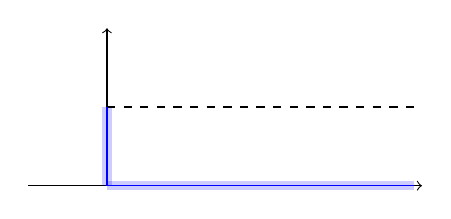
\begin{tikzpicture}
\draw[->] (-1,0) -- (4,0);
\draw[->] (0,1) -- (0,2);
\draw[color=blue] (0,1) -- (0,0);
\fill[opacity = 0.2, blue] (-0.4ex,0) -- (-0.4ex,1) -- (0.4ex,1) -- (0.4ex,0) -- cycle;
\fill[opacity = 0.2, blue] (0,-0.4ex) -- (3.9, -0.4ex) -- (3.9, 0.4ex) -- (0,0.4ex) -- cycle;
\draw[color=blue] (0,0) -- (3.9,0);
\draw[dashed] (0,1) -- (4,1);
\end{tikzpicture}
\caption{Representación gráfica de la unión de $S_1$ y $S_2$}
\end{figure}

\spart

\[\convx{S} = \{x = \sum^{n+1}λ_ix_i\;λ_i \geq 0, \sum λ_i = 1\; x_i\in S\}\]

Tomando \[k = \{(λ_1,λ_2,...,λ_{n+1},x_1,...,x_{n+1}) \;λ_i \geq 0, \sum λ_i = 1\; x_i\in S\}\]

Y construimos: $\appl{f}{k}{\convx{S}}$ tal que $f(λ_1,λ_2,...,λ_{n+1},x_1,...,x_{n+1}) = \sum^{n+1}λ_ix_i$ y esta función es continua.

Tenemos $k$ compacto (por ser $S$ compacto) y que  $f(k) =\convx{S}$, siendo $f$ continua.
%
Entonces, $\convx{S}$ es compacto (por ser imagen continua de un compacto).

\end{problem}

\begin{problem}[9]

Encuentra un ejemplo que muestre que la implicación

\[S_1,S_2 \text{ convexos cerrados} \implies S_1+S_2\text{ es cerrado}\]

no es cierta en general.
%
Prueba que esta implicación es cierta cuando al menos uno de los 2 conjuntos $S_1$ o $S_2$ se supone compacto.

\solution

\[S_1 = \{ (x_1,x_2) \in \real^2\tq\; x_2\geq \rfrac{1}{x_1} \;x_1 > 0\}\]
\[S_2 = \{(x_1,0) \in \real^2\tq x_1\in\real\}\]

Vamos a construir $S_1 + S_2$


\begin{figure}[hbtp]
\centering
\begin{tikzpicture}
\draw[->] (-1,0) -- (4,0);
\draw[->] (0,-1) -- (0,4);
\fill[opacity = 0.5,black,pattern=north east lines] (4,4) -- plot[variable=\t,samples=25,domain=0.25:4] (\t,1/\t);
\end{tikzpicture}
\caption{Representación gráfica de la suma de $S_1$ y $S_2$}
\end{figure}


\[S_1 + S_2  = \{(x_1,x_2)\tlq x_2>0\}\]

\[(0,0) = \lim (\underbrace{x_k}_{\in S_1} + \underbrace{y_k}_{S_2})\]

Para que sea la suma sea cerrada, necesitaríamos $\{y_k\},\{x_k\} \to (0,0)$ y en este caso no es así.
%
Vamos a ver que con que uno de los 2 conjuntos sea acotado, la suma ya es acotada.

\begin{prop}

$S_1,S_2$ convexos y cerrados, con $S_1$ acotado.

Tomamos $x_k + y_k \in S_1 + S_2$ y tenemos $\lim(x_k + y_k) = z$.

Entonces,
\[z\in S_1 + S_2\]
\end{prop}
\begin{proof}
Existe una subsucesión convergente $\{x_{k_i}\}$de $\{x_k\}$, por ser $S_1$ compacto.
Sea $\gor{x} = \lim x_{k_i}$, con $\gor{x}\in S_1$.

La correspondiente subsucesión de $y_k$ también converge (ya que sino la suma no puede converger)

\end{proof}

\end{problem}

\begin{problem}[10]

$S$ convexo es la intersección de todos los subespacios cerrados que lo contienen.

Formalmente:

\[S = \bigcap_{\begin{array}{c}S\subset H_i\\H_i\text{ compacto}\end{array}} H_i\]

\solution

$S\in \bigcap$ es trivial.

\[\left.\begin{array}{c} x\in\bigcap H_i\\x\not\in S \end{array}\right\} \implies \exists p≠0, α\in\real p^ty\leq α ∀y\in S p^t x >α\]


\end{problem}

\begin{problem}[11]

Sean $S_1,S_2$ dos conjuntos convexos no vacíos de $\real^n$ tales que $S_1\cap S_2 = \emptyset$.
Demuestra que existe $p ∈ \real^n , p≠0$, tal que

\[\inf\{p^Tx: x\in S_1\} \geq \sup\{p^Tx : x\in S_2\}\]

Si además, los conjuntos son cerrados y uno de ellos es acotado, demostrar que existe $\rho \in \real^n,\rho ≠ 0, ε > 0$ tales que

\[\inf\{p^Tx: x\in S_1\} \geq ε + \sup\{p^Tx : x\in S_2\}\]

\textit{Sugerencia: Para la primera parte, considera $S = \{x_1 - x_2 : x_1 \in S_1, x_2 \in S_2\}$ y aplica algún teorema de separación}

\solution


\[ S = \{x_1-x_2 \tq x_1\in S_1, x_2\in S\]

Es convexo, y tenemos $S_1\cap S_2 = 0 \implies 0\not\in S$.

Por ser $\gor{S}$ cerrado y convexo, tenemos 2 posibilidades $0\in S$ o $0\not\in S$:
\[0\not\in \gor{S}\implies \exists p≠0, \exists α\in ℝ p^tx\geq α>0 ∀x\in S\]

\[
\implies p^tx_1 \geq α + p^tx_2 ∀x_i\in S_i
\]


Si por el contrario:

\[
0\in \gor{S} - S \implies 0 \in \partial S \implies \exists p≠0, p^tx\geq 0, ∀x\in S
\]

Eso último se debe a $p^tx_1 ≥ p^tx_2, ∀x_i\in S_i$



\end{problem}

\begin{problem}[12]

\solution

\begin{defn}[Función\IS soporte]
\[S_c(p) = \sup\{p^tx\;:x\in C\}\]
La utilidad de la función soporte es poder comparar funciones en vez de trabajar con conjuntos.
%
Esto está muy bien porque en general es más fácil trabajar con funciones que con conjuntos sobretodo en temas de convergencia.
\end{defn}



Queremos probar que:

\[C = D \dimplies S_C(p) = S_D(p)\]

$\implies)$: Trivial

$\impliedby)$: Supongamos que existe $\gor{x}\in D \tlq \gor{x}\notin C$.
%
De esta manera, podemos aplicar un teorema de separación, es decir:

\[∃p≠0 \tlq p^tx≤α ∀x∃C \implies S_C(p) ≤α \wedge S_D(p) > α \]


\end{problem}

\begin{problem}[13]
Demuestra que si $x$ es una solución factible básica de $S = \{x : Ax = b, x ≥ 0\}$, entonces
es un punto extremo de S.

\solution

$x$ es una solución factible básica si al elegir una base, tenemos: \[x = \begin{pmatrix}B^{-1}b\\0\end{pmatrix} \equiv \begin{pmatrix}\gor{b}\\0\end{pmatrix}\]

Vamos a escribir $x$ como combinación convexa de puntos y ver que esos puntos son iguales a $x$, es decir:

\[\begin{pmatrix}B^{-1}b\\0\end{pmatrix} = λx_1 + (1-λ)x_2 = λ\begin{pmatrix}X_{1B}\\X_{1N}\end{pmatrix} + (1-λ)\begin{pmatrix}X_{2B}\\X_{2N}\end{pmatrix}\]

Como $x_1≥0,x_2≥0 \implies X_{1N} = X_{1B} = 0$.
%
Entonces, tenemos para $i=1,2$:

\[x_i = \begin{pmatrix}X_{iB}\\0\end{pmatrix} \implies Bx_{iB} + N0 = b \implies x_{iB}B^{-1}b = \gor{b}\]


\end{problem}


\begin{problem}[14]
Halla los puntos extremos de los siguientes conjuntos:

\ppart $S = \{(x_1,x_2) \in \real^2 : x_1 + 2x_2 \geq 2, -x_1+x_2 = 4, x_1,x_2\geq 0\}$
\ppart $S = \{(x_1,x_2,x_3) \in \real^3 : x_1 + x_2 + x_3 \leq 10, -x_1+2x_2 = 4, x_1,x_2,x_3\geq 0\}$

\solution

\spart
\label{ej:ejercicio2.14.a}
Aunque el problema se puede resolver sólo gráficamente, vamos a solucionarlo también algebraicamente.


\begin{figure}[hbtp]
\centering
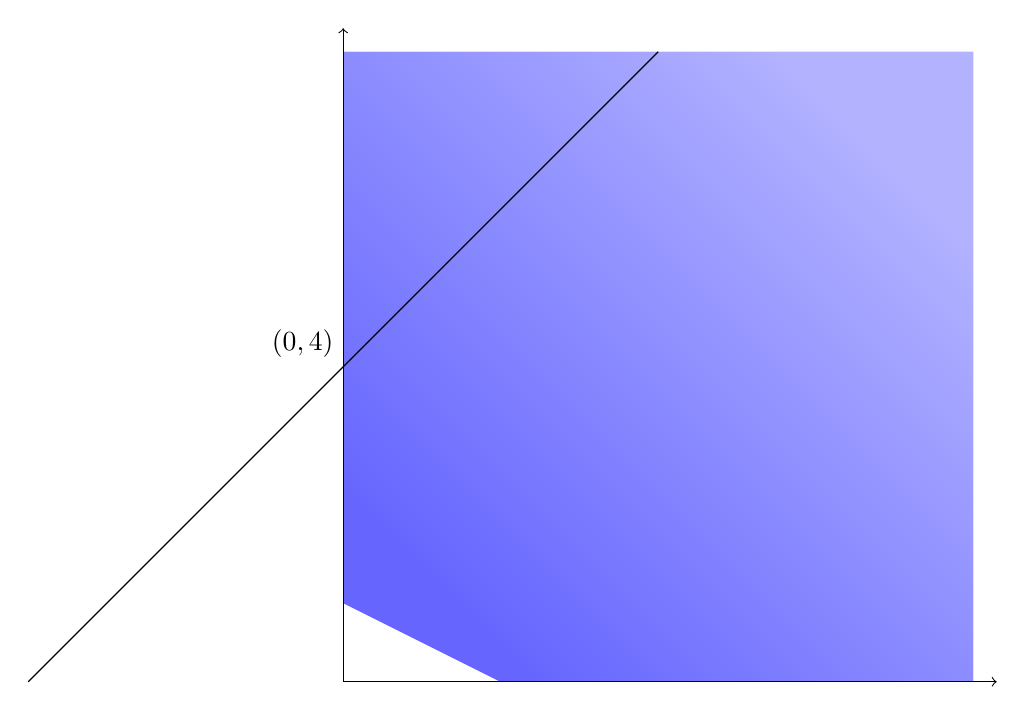
\begin{tikzpicture}
\fill[shading = axis,rectangle, left color=blue!60!white, right color=blue!30!white,shading angle=135,blue!60!white] (0,1) -- (2,0) -- (8,0) -- (8,8) -- (0,8);
\node[anchor=south east] at (0,4) {$(0,4)$};
\draw (-4,0) -- (0,4) -- (4,8);
\draw[->] (0,0) -- (0,8.3);
\draw[->] (0,0) -- (8.3,0);
\end{tikzpicture}
\caption{Solución gráfica del \fref{ej:ejercicio2.14.a}}
\end{figure}

Para resolverlo algebraicamente, tenemos que ir probando con las bases hasta obtener $\gor{b} ≥ 0$.
%
Lo primero que hay que hacer es reconstruir con las variables de holgura, es decir:

\[S = \{(x_1,x_2) \in \real^2 : x_1 + 2x_2 - x_3 = 2, -x_1+x_2 = 4, x_1,x_2,x_3\geq 0\}\]


La solución es:

\[
B = \begin{pmatrix}2&-1\\1&0\end{pmatrix} \implies \gor{b} = \begin{pmatrix}4\\6\end{pmatrix} ≥ \begin{pmatrix}0\\0\end{pmatrix}
\]

\spart

La solución gráfica está en \fref{fig:ejercicio2.14.b}. pero como antes: vamos a resolverlo algebraicamente. 

$S = \{(x_1,x_2,x_3) \in \real^3 : x_1 + x_2 + x_3 \leq 10, -x_1+2x_2 = 4, x_1,x_2,x_3\geq 0\}$

Tras escribirlo con igualdades, obtenemos:

\[
	A = \begin{pmatrix} 1&1&1&1\\-1&2&0&0\end{pmatrix}\;\; b = \begin{pmatrix}10\\4\end{pmatrix}
\]

Tenemos que probar las posibles bases que hay en $A$, para ello:

\[
	B = (a_1,a_2) = \begin{pmatrix}1&1\\-1&2\end{pmatrix} \to B^{-1}b = \begin{pmatrix}\rfrac{2}{3}&\rfrac{-1}{3}\\\rfrac{1}{3}&\rfrac{1}{3}\end{pmatrix} \begin{pmatrix}10\\4\end{pmatrix} = \begin{pmatrix}\rfrac{16}{3}\\\rfrac{14}{3}\end{pmatrix} \to SFB_1 = \begin{pmatrix}\rfrac{16}{3}\\\rfrac{14}{3}\\0\\0\end{pmatrix}
\]


\[
	B = (a_2,a_3)  = \begin{pmatrix}1&1\\2&0\end{pmatrix} \to B^{-1}b = \begin{pmatrix}0&\rfrac{1}{2}\\1&\rfrac{-1}{2}\end{pmatrix}\begin{pmatrix}4\\10\end{pmatrix} = \begin{pmatrix} 2\\8\end{pmatrix} \to SFB_2 = \begin{pmatrix} 0\\2\\8\\0\end{pmatrix}
\]

\[
	B = (a_1,a_3) = (a_1,a_4) = \begin{pmatrix} 1&1\\-1&0\end{pmatrix} \to B^{-1}b = \begin{pmatrix}0&-1\\1&1\end{pmatrix}\begin{pmatrix}4\\10\end{pmatrix} = \begin{pmatrix}\textcolor{red}{-4}\\14\end{pmatrix} \to \text{no es } SFB
\]

\[
	B = (a_2,a_4) \to SFB_3 = \begin{pmatrix}0\\2\\0\\8\end{pmatrix}
\]


\begin{figure}[hbtp]
\centering
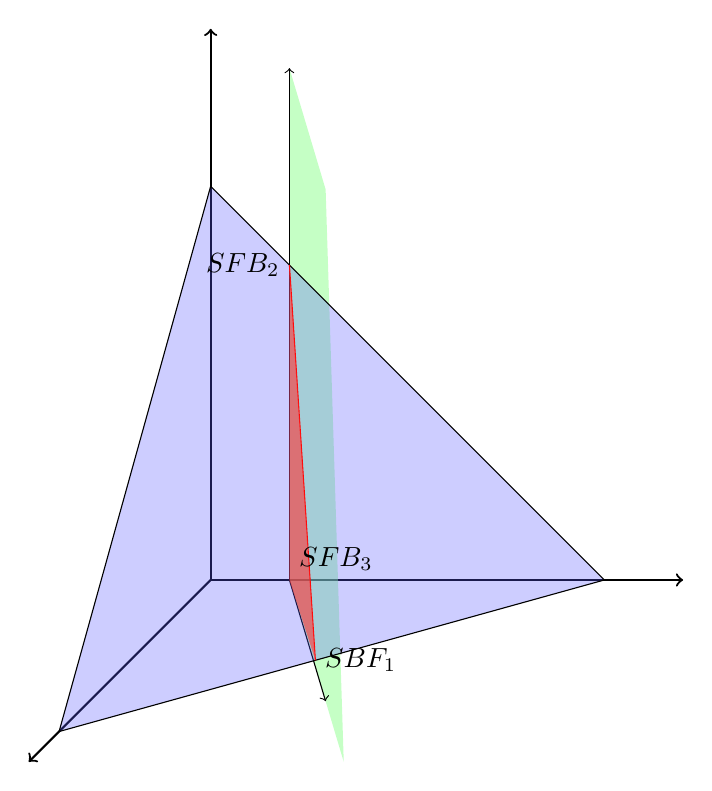
\begin{tikzpicture}[scale=0.5]
\draw[->,thick] (0,0,0) -- (0,0,12); %% X
\draw[->,thick] (0,0,0) -- (12,0,0); %% Y
\draw[->,thick] (0,0,0) -- (0,14,0); %% Z
\fill[green!45!white,opacity=0.5] (6,13,8) -- (8,0,12)  -- (2,0,0) -- (2,13,0) -- cycle;
\draw[->] (2,0,0) --  (6,0,8);
%\draw[->] (0,0,4) --(0,13,4);
\draw[->] (2,0,0) -- (2,13,0);
\fill[blue!65!white,opacity=0.3] (10,0,0) -- (0,10,0) -- (0,0,10) -- cycle;
\draw (10,0,0) -- (0,10,0) -- (0,0,10) -- cycle;
\draw[red] (2,8,0) -- (4.7,0,5.3);
\fill[red!80!white,opacity=0.6] (2,0,0) -- (4.7,0,5.3) -- (2,8,0) -- cycle;
\node[right] at (4.7,0,5.3) {$SBF_1$};
\node[left] at (2,8,0) {$SFB_2$};
\node[above right] at (2,0,0) {$SFB_3$};
\end{tikzpicture}
\caption{Por debajo del plano azul, la primera restricción. En verde la segunda restricción, con lo que en rojo tenemos el conjunto factible con 4 puntos extremos.}
\label{fig:ejercicio2.14.b}
\end{figure}
\end{problem}


\section{Hoja 3}

\begin{problem}[1]

Resolver utilizando el algoritmo de simplex el problema:

\begin{ioprob}
\goal{$x_2 - 3x_3 + 2x_5$}
\restrictions{$x_1+3x_2-x_3+2x_5 = 7$}{$-2x_2 + 4x_3 + x_4 = 12$}{$-4x_2 + 3x_3 + 8x_5 + x_6 = 10$}{$x_i \geq 0$}{}
\end{ioprob}

\solution

Vamos a construir la tabla del simplex:


\begin{table}[hbtp]
\centering
\begin{tabular}{c|cccccc}
$c_j$&0&1&-3&0&2&0\\\hline
Variables & $x_1$&$x_2$&$x_3$&$x_4$&$x_5$&$x_6$\\\hline
7&1&3&-1&0&2&0\\
12&0&-2&\textcolor{red}{4}&1&0&0\\
10&0&-4&3&0&8&1\\\hline
$z_j - c_j$ & 0&-1&3&0&-2&0
\end{tabular}
\end{table}

Incluimos la solución final, para terminar el problema en casa.
%
Tras 2 iteraciones obtenemos:


\begin{table}[hbtp]
\centering
\begin{tabular}{c|cccccc}
\hline
4&$\rfrac{2}{5}$&1&0&0.1&0.8&0\\
5&0.2&0&1&0.3&0.4&0\\
11&1&0&0&-0.5&10&1\\\hline
&-0.2&0&0&-0.8&$-\rfrac{12}{5}$&0
\end{tabular}
\end{table}

Entonces, la solución sería:

\[
\gor{x} = (0,4,5,0,0,11)
\]
\end{problem}

\begin{problem}

\solution
\todoby{Parra}
\end{problem}

\begin{problem}[3]
Consideremos el siguiente problema de optimizaci\'on lineal:

\begin{center}
\begin{tabular}{ll}
Minimizar & $c_1x_1+c_2x_2+c_3x_3$ \\
sujeto a & \\
& $x_1 - x_2 + 5x_3\leq 10$\\
& $2x_1 - x_2 + 3x_3 \leq 40$\\
&$x_1\geq 0,\ x_2\geq 0,\ x_3\geq 0$
\end{tabular}
\end{center}


\ppart Calcula una direcci\'on extrema  y dos puntos extremos
  del conjunto factible.
\ppart Determina unos coeficientes $c_1,c_2,c_3$
de la funci\'on objetivo tales que el problema no tenga
soluci\'on \'optima finita.
\ppart Determina unos coeficientes $c_1,c_2,c_3$
de la funci\'on objetivo tales que el problema tenga
infinitas soluciones \'optimas.



\solution

Lo primero es escribir el problema en forma estándar:


\begin{ioprob}
\goal{$\min \sum_{i=1}^3 c_ix_i$}
\restrictions{$x_1-x_2+5x_3 + x_4 = 10$}{$2x_1 - x_2 + x_3 + x_5 = 40$}{$x_i \geq 0$}{}{}
\end{ioprob}

\spart

Cogemos una base y operamos:

\[B = \begin{pmatrix}1&0\\0&1\end{pmatrix} \to B^{-1}b = b = \begin{pmatrix}10\\40\end{pmatrix}\geq \begin{pmatrix}0\\0\end{pmatrix} \to (0,0,0,10,40)\]

Como $B^{-1}b \geq 0$, $(0,0,0,10,40)$ es un punto extremo.

Tomando por ejemplo:

\[B = \begin{pmatrix}5&0\\3&1\end{pmatrix} \to ... \to (0,0,2,0,34)\]

Obtenemos otro punto extremo.

\textbf{Dirección extrema}

\[
B=
	\begin{pmatrix}
	1&0\\
	0&1
	\end{pmatrix}\;\;
a_j = a_2\implies B^{-1}a_2 =
\begin{pmatrix}
-1\\
-1
\end{pmatrix}\geq
\begin{pmatrix}
0\\
0
\end{pmatrix} \to d = α
\begin{pmatrix}
0\\
1\\
0\\
\hline 1\\1
\end{pmatrix}\]

\spart

Para cualquier $c_1,c_3$, mientras tomemos $c_2$ negativo no vamos a tener nunca una solución óptima.

\spart

Para tener infinitas soluciones óptimas, necesitamos vectores de coeficientes distintos que nos den el mismo valor objetivo.

Podemos tomar $c_1,c_2,c_3$ de tal manera que los 2 puntos extremos que tenemos calculados antes tengan el mismo valor objetivo.
%
De esta manera,  el segmento que une los 2 puntos tiene el mismo valor objetivo.
\end{problem}


\begin{problem}[4]

Dado un problema de optimización lineal $\min c^\top x$, sujeto a $Ax = b, x ≥ 0$, ¿es posible conseguir un
problema en el que no exista solución óptima finita cambiando únicamente el vector b? Responde a
la misma pregunta para el vector c

\solution

Los teoremas de caracterización nos daban una condición de existencia de solución en caso de cosas en las que no influye $b$, por lo que $b$ no influye y por lo tanto no es posible conseguirlo.

En cuanto al $c$, simplemente con cambiarlo de signo se revienta todo.

\end{problem}

\begin{problem}[5]

Consideremos el problema de optimizaci\'on
\begin{equation*}
	{\rm min}\ z=c^\top x\ \ \hbox{sujeto a}\ \ x\in S=\{x\in\mathbb{R}^n:\, Ax= b,x\geq 0\}
\end{equation*}
donde $b\in\mathbb{R}^m$, $c\in\mathbb{R}^n$ y $A$ es una matriz $m\times n$ de rango $m$.



\ppart Supongamos que $S≠\emptyset$ y que para un cierto vector no nulo d ≥ 0, $d∈\real^n$ , se verifica $Ad = 0$ ¿Puede asegurarse entonces que existe un vector $c≠0$ tal que el problema tiene solución
óptima no acotada?

\ppart ¿Puede ocurrir que una solución óptima tenga más de m componentes estrictamente positivas?

\ppart Si $\gor{x}\in S$ tiene exactamente m componentes estrictamente positivas, ¿puede asegurarse que $\gor{x}$ es un punto extremo de S?



\solution

\spart
Como $S≠\emptyset$, tenemos $\gor{x}\in S$ y tal que $\gor{x} + λd\in S ∀λ>0$ ya que $A(\gx + λd) = A\gx + λAd = A\gx \in S$.

Esto quiere decir que hay una dirección extrema, en la que a lo largo de ella, nunca salimos del conjunto factible.
%
Basta tomar un $c$ que haga que en esa dirección mejore el valor objetivo, para que la solución no esté acotada.
%
Podemos tomar cualquier $c$ tal que $c^\top d<0$, por ejemplo $c=-d$.

De esta manera, para cualquier $\gx$ que cumpla $Ax=b$, tenemos $∀λ>0,\; A(\gx+λd) = A\gx+λAd = A\gx = b$, cuyo valor objetivo es: $-d^\top(\gx+λd) = -d^\top \gx -λd^\top d < 0$. Podemos tomar $λ$ tan grande como queramos, dando lugar a una solución no acotada.


\spart Claro que puede ocurrir.

\spart Sabemos que punto extremo $\dimplies$ solución factible básica.
%
No puede asegurarse, ya que podemos fijar $n-m$ coordenadas iguales a $0$.
%
Si las otras $m$ no forman una base, no podemos despejar para tener un punto extremo.
%
Por ejemplo:


\begin{ioprob}
\goal{}
\restrictions{$x_1+x_3+x_4 = 1$}{$x_2+x_3+x_4=1$}{$x_i≥0$}{}{}{}
\end{ioprob}

En este problema tenemos $n=4$ y $m=2$.
%
El punto $p = \left(0,0,\rfrac{1}{2},\rfrac{1}{2}\right)$ tiene exactamente 2 coordenadas positivas.
%
No es una $SFB$ por lo que no es un punto extremo.

No es una $SFB$ porque $a_3 = a_4 = \begin{pmatrix}1\\1\end{pmatrix}$, por lo que $\{a_3,a_4\}$ no forman una base.

\end{problem}


\begin{problem}[6]

Consideremos el problema:
maximizar $x_1+3x_2+x_3$, sujeto a $Ax\leq b$, $x\geq 0$,
siendo $A$ una matriz $2\times 3$, $b\in\mathbb{R}^2$ ($b\geq 0$) y
$x=(x_1,x_2,x_3)^\top$.
Se resuelve este problema pas\'andolo a forma est\'andar
(para lo cual se a\~naden dos variables de holgura $x_4$ y $x_5$) y
aplicando el algoritmo del simplex. La tabla final del algoritmo ha
sido:

\begin{center}
\begin{tabular}{c||c|c|c|c|c}
$c_j$&-1&-3&-1&0&0\\
\hline
Variables&$x_1$&$x_2$&$x_3$&$x_4$&$x_5$\\
\hline
$x_1=12$&1&4&3&1&0\\
$x_5=16$&0&6&2&1&1\\
\end{tabular}
\end{center}

\ppart Calcula la matriz $A$ y el vector $b$.

\ppart Supongamos que el vector de costes $c = (1, 3, 1, 0, 0)$ se reemplaza por $c^\top = c + λγ$, siendo λ un número no negativo e $γ = (1, 1, 1, 0, 0)$. ¿Para qué valores de λ sigue siendo solución óptima $x = (12, 0, 0, 0, 16)$ ?

\solution

\spart

Cada columna $y_j = B^{-1}a_j$.
%
Si conociéramos $B^{-1}$, ya tendríamos todo.
%
Vamos a descubrir $B$.

\[
	\left.\begin{array}{c}
		y_4 = B^{-1}\begin{pmatrix}1\\0\end{pmatrix} = \begin{pmatrix}1\\1\end{pmatrix}\\
		y_5 = B^{-1}\begin{pmatrix}0\\1\end{pmatrix} = \begin{pmatrix}0\\1\end{pmatrix}
	\end{array}\right\} \implies B^{-1} = \begin{pmatrix}1&0\\1&1\end{pmatrix} \implies B = \begin{pmatrix}1&0\\-1&1\end{pmatrix}
\]

Ahora podemos calcular:

\[
	a_j = By_j \implies
	\left\{
		\begin{array}{c}
			a_2 = \begin{pmatrix}4\\2\end{pmatrix}\\
			a_3 = \begin{pmatrix}3\\-1\end{pmatrix}\\
		\end{array}
	\right.
\]

Con esto:

\[
	A =
		\begin{pmatrix}
			1&4&3&1&0\\
			-1&2&-1&0&1
		\end{pmatrix}
\]

\textbf{Otra posibilidad}

\[
	\begin{pmatrix} 1&4&3&1&0 \\ 0&6&2&1&1 \end{pmatrix} \overset{Gauss}{\to} \left(\begin{array}{c|c} Λ & \begin{array}{cc}1&0\\0&1\end{array}\end{array}\right) = A
\]

\spart Si el problema es de maximización, la tabla es óptima si $z_j - c_j ≥ 0 ∀j∈ℕ$.

El caso general, para un $\gamma$ dado sería:

\begin{align*}
	\hat{z_j} - \hat{c_j} = \hat{c}^\top y_j - \hat{c}_j &= (c^t_B + λ\gamma_B)'y_j - (c_j + λ\gamma_j) = (c_B^\top y_j - c_j) + λ(\gamma^\top_By_j - \gamma_B) =
\end{align*}
\begin{align*}
	 \underbrace{(z_j - c_j)}_{≥0} + λ(\gamma_By_j - γ_j) &\overset{?}{≥} 0 ∀j∈ℕ
\end{align*}

Mientras se mantenga la desigualdad, tendremos solución óptima.

Si $∀j∈ℕ$, entonces la desigualdad se mantiene ya que $(\gamma_By_j - γ_j) ≥ 0 $.
%
Además, se mantiene $∀λ$.

Si $∃j∈ℕ\tq γ_b^\top y_j - γ_j < 0$, entonces $λ$ no puede tomar cualquier valor positivo.
%
Como máximo, $λ = \min\{\text{algo}\}$. ¿Cuánto podemos aumentar $λ$?

\[λ ≤ \min\left\{  \frac{z_j - c_j}{-(γ_B^\top y_j - γ_j)} \right\}\]

Para este caso concreto (en el que estamos maximizando y no minimizando, con lo que hay un signo que no cambiamos)

\[
	γ_B = (1,0)' \to
	(1,0)y_j - γ_j =
	\begin{pmatrix}
		4-1 = 1\\
		3-1 = 2\\
		1-0 = 1
	\end{pmatrix}
\]


\end{problem}


\begin{problem}[7]
Considera la siguiente tabla del simplex para un
problema  lineal de minimizaci\'on ($a,b,c,d$ y $e$
denotan aqu\'{\i} par\'ametros reales):

\begin{center}
\begin{tabular}{c||c|c|c|c|c}
$c_j$&0&b&e&0&0\\
\hline
Variables&$x_1$&$x_2$&$x_3$&$x_4$&$x_5$\\
\hline
$x_1=a$&1&c&3&0&0\\
$x_4=2$&0&d&2&1&0\\
$x_5=4$&0&-1&1&0&1\\
\end{tabular}
\end{center}


Determina condiciones sobre los par\'ametros $a,b,c,d$ y $e$ de manera que

\ppart  La tabla corresponda a una soluci\'on \'optima.
\ppart  La tabla indique la situaci\'on de \textit{soluci\'on \'optima no acotada}.
\ppart  La tabla corresponda a una soluci\'on \'optima y la regi\'on factible  no sea acotada.

\obs Este es un problema de examen (ligeramente cambiado)


\solution

a≥0 (está en la pizarra pero no se de donde sale).

\spart

En este caso, $\gor{z_j} = z_j - c_j = -c_j$, si $a_j∈B$. 
%
Para que sea solución óptima, $\gor{z_j} ≥ 0$, con lo que:

\[ z_2 - c_2 = -b ≤ 0 \implies b≥0\]
\[ z_3 - c_3 = -e ≤ 0 \implies e≥0\]

\spart $b<0$ para que el valor objetivo mejore al aumentar $x_2$ y $c,d≤0$ para que podamos aumentar todo lo que queramos.

Si $b=0$, con $c,d≤0$ podemos aumentar  

\spart $b,e≥0$ para que sea óptima y para tener una dirección extrema, necesitamos $c,d≤0$.

\end{problem}

\begin{problem}[8]
Demuestra que, en el algoritmo del simplex, una variable que sale de la base en una determinada
iteración no puede volver a entrar en la base en la iteración inmediatamente posterior.
\solution

\[\hat{z_r} - \hat{c_r} = \underbrace{(z_r - c_r)}_{0} - \underbrace{\frac{y_{rr}}{y_{r_k}} (z_k - c_k)}_{<0}\implies (1)\]

$(1)$  la variable $r$ no entra en la siguiente iteración (aunque más adelante si podría volver a entrar).

\begin{itemize}
\item Como $r$ era una variable de la base, teníamos $z_r - c_r = 0$.
\item $y_{r_k} > 0$ por ser el pivote.
\item $y_{rr} = 1$ ya que la columna del elemento r de la base es $(0,0,...,0,1,0,...,0)$ en la posición $r$.
\item $z_k - c_k > 0$ ya que la variable $k$ entró en la base.
\end{itemize}

\end{problem}

\begin{problem}

Estudia cómo puede detectarse mediante el algoritmo del simplex la existencia de “alternativa óptima”, es decir, la existencia de más de una solución óptima.
\solution

Si estamos en el óptimo, tenemos $z_j - c_j ≤ 0 ∀j∈N$. ¿Cómo descubrir que el óptimo no es único?

La condición de optimalidad es:

\[z = \bar{z} = \sum_{j∈N}(z_j - c_j)x_j\]

Es condición necesaria que exista $j∈N$, tal que $z_j - c_j = 0$.
%
De esta manera, al aumentar $x_j$ no aumenta el valor objetivo y tenemos infinitas soluciones óptimas.

Vamos a ver un ejemplo:

\begin{ioprob}
\goal{$\min\{-x_1-x_2\}$}
\restrictions{$x_1+x_2 ≤ 6$}{$x_1≤3$}{$x_1,x_2 ≥ 0$}{}{}{}
\end{ioprob}

\begin{figure}[hbtp]
\centering
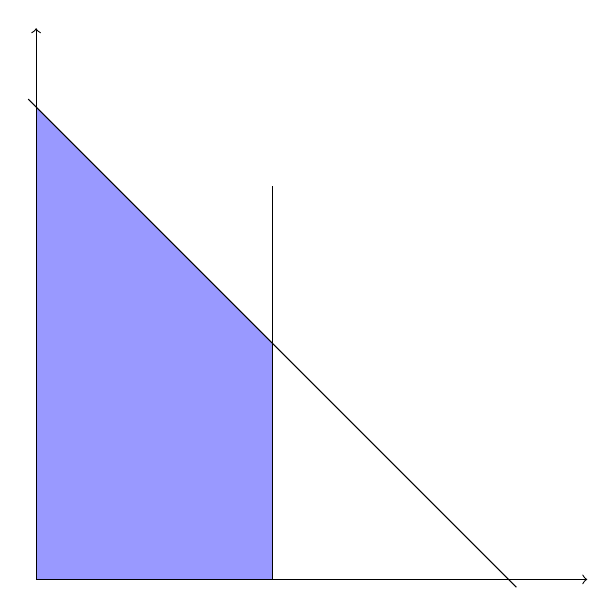
\begin{tikzpicture}
\fill[fill=blue!40!white](0,0) -- (3,0) -- (3,3) -- (0,6) -- (0,0);
\draw[->] (0,0) -- (7,0);
\draw[->] (0,0) -- (0,7);
\draw (3,0) -- (3,5);
\draw (6.1,-0.1) -- (-0.1,6.1);

\end{tikzpicture}
\caption{Solución gráfica del problema.}
\end{figure}



Vamos a construir el algoritmo del simplex, pasando previamente el problema a forma estándar:

\begin{table}[hbtp]
\centering
\begin{tabular}{c|cccc}
$c_j$ & -1 & -1 &0&0\\\hline\hline
6&1&1&1&0\\
3&1&0&0&1\\\hline
$z_j - c_j$ & 1&1&0&0
\end{tabular}
\end{table}


\begin{table}[hbtp]
\centering
\begin{tabular}{c|cccc}
$c_j$ & 0 & 1 & 1 & -1\\\hline\hline
3 & 0 & 1 & 1 & -1 \\
3 & 1 & 0 & 0 & 1 \\\hline
$z_j - c_j$ & 0&0&-1& \textcolor{red}{0}
\end{tabular}
\end{table}


El punto solución son de la forma $(3,3,0,0)$, pero si tomamos $(3-α,3+α,0,α)$ (es decir, entra la 4º variable), seguimos teniendo un punto óptimo. ¿Hasta que valor puede llegar $α$? $α=3$ como máximo, entonces obtendríamos puntos óptimos de la forma $(0,6,0,3)$.

Volviendo a la pregunta. \textbf{¿Condición necesaria y no suficiente?} Vamos a hacer un ejemplo en el que realmente veamos esto.


\begin{ioprob}
\goal{$\min\{x_1\}$}
\restrictions{$x_1-x_2 ≤ 0$}{$2x_1 - x_2≥0$}{$x_1,x_2 ≥ 0$}{}{}{}
\end{ioprob}

Gráficamente el problema:

\begin{figure}[hbtp]
\centering
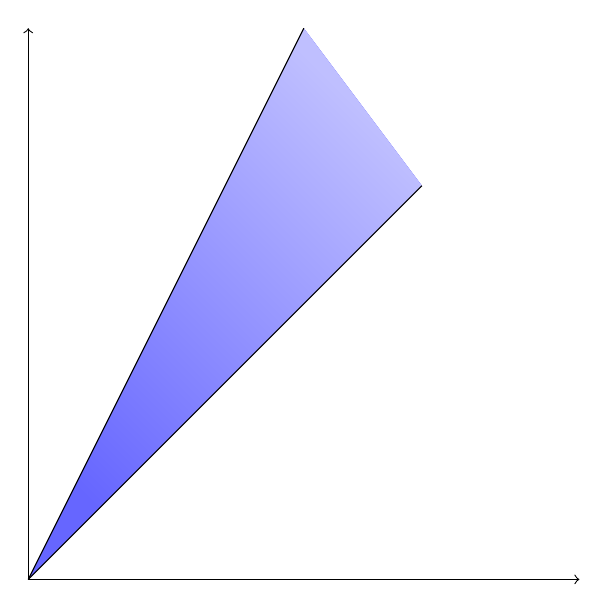
\begin{tikzpicture}
\fill[shading = axis,rectangle, left color=blue!60!white, right color=blue!25!white,shading angle=135,blue!75!white] (0,0) -- (5,5) -- (3.5,7) -- (0,0);
\draw[->] (0,0) -- (7,0);
\draw[->] (0,0) -- (0,7);
\draw (0,0) -- (5,5);
\draw (0,0) -- (3.5,7);
\end{tikzpicture}
\caption{Solución gráfica del problema.}
\end{figure}


Vamos a resolverlo con simplex.
%
Para ello, convertimos el problema en forma estándar:

\begin{ioprob}
\goal{$\min\{x_1\}$}
\restrictions{$x_1-x_2 +x_3= 0$}{$-2x_1 + x_2 + x_4 = 0$}{$x_1,x_2,x_3,x_4 ≥ 0$}{}{}{}
\end{ioprob}

La tabla del simplex sería:

\begin{table}[hbtp]
\centering
\begin{tabular}{c|cccc}
$c_j$ & 1 & 0 & 0 & 0\\\hline\hline
0 & 1 & -1 & 1 & 0 \\
0 & -2 & 1 & 0 & 1 \\\hline
$z_j - c_j$ & -1 & 0 & 0 & 0
\end{tabular}
\end{table}

Y vemos que ya hemos acabado, porque son todas negativas o $0$.
\end{problem}

\begin{problem}
En una iteración del algoritmo del simplex aplicado a un problema lineal de minimización se
obtiene la tabla siguiente:

\begin{centering}
\begin{tabular}{c|cccc}
&-2&3&0&0\\\hline
&$x_1$&$x_2$&$x_3$&$x_4$\\\hline
$x_3 = 4$ & c&0&1&$\rfrac{1}{5}$\\
$x_1 = a$ & d&e&0&2\\\hline
&f&-1&g&h
\end{tabular}
\end{centering}

El valor del objetivo del problema en la solución básica factible a la que corresponde la tabla
anterior es -6.
%
Las variables $x_3$ y $x_4$ son de holgura y formaban la base inicial.

\ppart Calcula el valor de las siete incógnitas a, c, d, e, f , g y h.

\ppart ¿Corresponde la tabla a una solución básica factible óptima?
\solution

\spart $c=0$,$d=1$,$f=g=0$.

\[h = z_4 - c_4 = c^\top_By_4 - c_4 = (0,-2) \begin{pmatrix}\rfrac{1}{5}\\2\end{pmatrix} - 0  = --4 \]

\[ \bar{z} = -6 = -2a \implies a=3 \]

\spart  Sí, porque son todos $0$ o negativos.

\end{problem}

\begin{problem}[11]

\solution

La condición de optimalidad no depende de $b$, entonces se sigue cumpliendo si $b\to b+θd$

\[
	B^{-1}b \to B^{-1}(b+θd) ≥ 0 \implies (b+θd)≥ 0 \implies \bar{d}≥0
\]
\begin{itemize}
	\item $\bar{d}≥0$, la base es óptima $∀θ≥0$.
	\item $\displaystyle\bar{d}\not ≥0 \implies b_i ≥ -θ\bar{d_i} \implies θ < \min\left\{\frac{-\bar{b_i}}{\bar{d}_i}\right\}$
\end{itemize}

\end{problem}


\section{Hoja 4}


\begin{problem}[1]
\label{ejer:h4e1}

Sea  $D\subset\mathbb{R}^n$ un conjunto convexo, y sea $f:D\to \mathbb{R}^n$ una funci{\'o}n definida sobre {\'e}l. 


\ppart Demuestra que una condici{\'o}n necesaria, pero no suficiente, para que $f$ sea convexa es que, para cada n{\'u}mero real $\alpha$, el conjunto $\{x\in D:\ f(x)\leq \alpha\}$ sea convexo. 
%
Es decir, demostrar $f$ convexa $\implies$ $S_{\alpha}$ es convexo $\forall \alpha$

Dar un contra ejemplo para la implicación recíproca.

\ppart $f$ convexa $\dimplies \epigraph(f)$ es un conjunto convexo.

\solution

\spart $f(x) = x^3$  es un contraejemplo válido para el recíproco.

\spart Recordamos que $\epigraph(f) = \{(x,t) : f(x) \leq t\}$

$\implies)$ Sean $(x_1,t_1),(x_2,t_2)\in \epigraph(f)$, para $\lambda \in [0,1]$ tomamos:

\[
 f(\lambda x_1 + (1-\lambda) x_2) \leq \lambda f(x_1) + (1-\lambda) f(x_2) \leq \lambda t_1 + (1-\lambda t_2)
 \]

Además, $\lambda t_1 + (1-\lambda t_2) \in \epigraph(f)$


$\impliedby)$ Tenemos 2 puntos de la función.
%
Si el segmento que los une es mayor que lo que vale la función, entonces la función es convexa.
%
Más formalmete:

\[
    (x_1,f(x_1)),(x_2,f(x_2)) \in \epigraph(f) \implies \left(\lambda (x_1,f(x_1)) + (1-\lambda) (x_2,f(x_2))\right) \in \epigraph(f) \implies\]
    \[ \lambda f(x_1) + (1-\lambda) f(x_2) \geq f(x_1 + (1-\lambda) x_2) \dimplies convexa
\]


\end{problem}

\begin{problem}[2]
Se dice que una función $f:\mathbb{R}^n\to\mathbb{R}$ es cuasiconvexa si los conjuntos $S_\alpha=\{x\in\mathbb{R}^n:\, f(x)\leq \alpha\}$ son convexos para todo $\alpha\in\mathbb{R}$. Demuestra que  $f$ es cuasiconvexa si y solo si para todo $x,y\in\mathbb{R}^n$ y $\lambda\in [0,1]$ se verifica $f((1-\lambda)x+\lambda y)\leq \max\{f(x),f(y)\}.$ 

\label{ejer:h2.e9}

\solution

$\implies)$ Tomando $\alpha=  \max\{f(x_1),f(x_2)\}$, como
$x_1,x_2 \in S_{\alpha} \implies \lambda x_1 + (1-\lambda) x_2 \in S_{\alpha}$ por ser $S_α$ convexo

Además, \[f(\lambda x_1 + (1-\lambda) x_2) \leq \alpha \implies \lambda x_1 + (1-\lambda) x_2 \in S_{\alpha} \]


$\impliedby)$ Tenemos $x_1,x_2 \in S_{\alpha},\lambda \in [0,1]$.

Dado $\lambda x_1 + (1-\lambda) x_2 \overset{?}{\in} S_{\alpha}$. 
%
Por hipótesis $f(\lambda x_1 + (1-\lambda) x_2) \leq \max\{f(x_1),f(x_2)\}$.

Tenemos que $∀x,y S_\{\max\{f(x),f(y)\}$ es convexo. 
%
Pero lo que necesitamos es $∀α S_α$ convexo.

Si $α\in\img f\to \exists x\tq f(x) = α$, con lo que $S_α$ convexo.
%
Si $α\notin \img f \to \nexists x\tq f(x) = α$, con lo que $S_α = \emptyset$ convexo.

\end{problem}

\begin{problem}[3]

\ex Comprueba si las siguientes funciones son convexas o cóncavas (o ni convexas ni cóncavas) en su dominio de definición:


\ppart $f(x_1,x_2,x_3)=(x_1+2x_2-3x_3)^2$.
\ppart $f(x_1,x_2)=8x_1-6x_2-2x_1^2-3x_2^2+4x_1x_2$.
\ppart $f(x_1,x_2)=\min\{x_1,x_2\}$.
\ppart $f(x_1,x_2)=(x_2-x_1^2)^2$.

\solution

\spart Es convexa por ser una composición de una función lineal con una función convexa.

\ppart Calculamos la matriz hessiana y comprobamos si es semidefinida positiva.

\[
\Hf{x_1,x_2,x_3} = \begin{pmatrix}	
-4&4\\4&-6
\end{pmatrix}
\]

Aplicamos el criterio de los menores principales.

Como el primer menor $\Delta_1 = -4 < 0$ y $\Delta_2 = \left|\begin{array}{cc}-4&4\\4&-6\end{array}\right| > 0$ entonces $\Hf{x_1,x_2,x_3}$ es definida negativa por lo que $f$ es estríctamente cóncava.


\ppart $f(x_1,x_2) = \min\{x_1,x_2\}$ es cóncava, ya que $\min\{x_1,x_2\} = -\max\{x_1,x_2\} $ y $\max\{x_1,x_2\}$ es convexa.

\ppart La matriz hessiana no es definida nada.
%
Podríamos restringirnos a subdominios en los que estudiar la función.
%
Igual hay un intervalo en el que la función sí es convexa.
\end{problem}


\begin{problem}[4]



\ex Sea $I\subset \mathbb{R}$ un intervalo y $f:I\to\mathbb{R}$ una función convexa.

\ppart (Lema de las tres cuerdas)  Sean $x,y,z\in I$ con $x<y<z$, demuestra
\[
\frac{f(y)-f(x)}{y-x}\leq \frac{f(z)-f(x)}{z-x}\leq \frac{f(z)-f(y)}{z-y}.
\]
Deduce que la función $g(x)=(f(x)-f(a))/(x-a)$, definida para $x\neq a$, es creciente.
\ppart Sea $c$ un punto del interior de $I$. Demuestra que existen las derivadas por la derecha y por la izquierda de $f$ en $c$ y verifican $f'_-(c)\leq f'_+(c)$.
\ppart Sean $a$ y $b$ puntos del interior de $I$ con $a<b$ entonces, por el apartado (b), existen las derivadas por la derecha y por la izquierda de $f$ en $a$ y $b$. Demuestra que se verifica:
\[
f'_-(a)\leq f'_+(a)\leq \frac{f(b)-f(a)}{b-a} \leq f'_-(b)\leq f'_+(b).
\]
\ppart Si $f$ es derivable, demuestra que $f$ es convexa si y solo si $f'$ es creciente.
\ppart Si $f$ es derivable dos veces, demuestra que $f$ es convexa si y solo si $f''(x)\geq 0$, para todo $x\in I$.


\solution

\begin{lemma}[Lema\IS de las 3 cuerdas]
Sea $\appl{f}{I}{\real}$ con $f$ convexa e $I\subset \real$.
%
Sean $x,y,z \in I$, $x<y<z$.
%
Entonces

\[
\frac{f(y)-f(x)}{y-x} \leq \frac{f(z)-f(x)}{z-x} \leq \frac{f(z)-f(y)}{z-y}
\]
\end{lemma}


\begin{figure}[hbtp]
\centering
\begin{tikzpicture}[scale=0.6]
\draw[thick,->] (-1,0) -- (8.5,0) node[anchor=west] {$x$};
\draw[thick,->] (0,-1) -- (0,10.5) node[anchor=east] {$y$};
\draw (2,2) node[point,anchor=north]  {$x$};
\draw (3,1) node[point,anchor=north]  {$y$};
\draw (4.75,4) node[point,anchor=west]  {$z$};
\draw plot[variable=\t,samples=25,domain=-2.25:3] (\t+3,\t*\t+1);
\draw[thick,-] (2,2) -- (3,1);
\draw[thick,-] (3,1) -- (4.75,4);
\draw[thick,-] (2,2) -- (4.75,4);
\end{tikzpicture}
\caption{Representación gráfica del lema de las 3 cuerdas.}
\end{figure}

\begin{proof}

\end{proof}

\obs En realidad, con que $f$ sea creciente debería ser suficiente.
%
Se deja como ejercicio la comprobación.

\ppart Las funciones convexas no pueden tener saltos en su dominio.

La clave en este ejercicio es utilizar el lema para decir que un cociente incremental de una función creciente y acotada (o decreciente y acotada, en el caso análogo) tenemos que existen las derivadas laterales.

\end{problem}

\begin{problem}[5]
Utiliza la desigualdad de Jensen (aplicada a una función convexa adecuada) para demostrar que si $x_1,\ldots,x_m \in\mathbb{R}$ y $\lambda_1,\ldots,\lambda_m>0$ con $\lambda_1+\cdots + \lambda_m=1$, entonces
\[
\prod_{i=1}^m x_i^{\lambda_i} \leq \sum_{i=1}^m \lambda_i x_i.
\]

\solution

\end{problem}

\begin{problem}[6]

Una función $f$ es log-convexa si es positiva y $\log f$ es convexa. Demuestra que toda función log-convexa es convexa. Demuestra que la función gamma, $\Gamma(x)=\int_0^\infty t^{x-1} e^{-t} dt$, $x>0$, es log-convexa (\textit{Indicación: usa la desigualdad de Hölder}).

\solution

\end{problem}

\begin{problem}
Sea $f:[0,\infty)\to\mathbb{R}$ convexa y derivable. Demuestra que la función que da los promedios de $f$ sobre los intervalos $[0,x]$, es decir $F(x)=(1/x)\int_0^x f(t)dt$, también es convexa.  (\textit{Indicación: calcula $F''(x)$ y exprésala en la forma $F''(x)=(2/x^3)\int_0^x g(x,t)dt$, para cierta función $g(x,t)$}).
\solution

\end{problem}

\begin{problem}[8]

Considera el problema $\min f(x)$ s.a. $x\geq 0$, donde $f:\mathbb{R}^n\to \mathbb{R}$ es convexa y diferenciable. Demuestra que $\bar{x}$ es la solución factible óptima de este problema si y solo si  para todo $i=1\ldots,n$ se cumple $\bar{x}_i\geq 0$,  $f'_i(\bar{x})\geq 0$ y $\bar{x}_if'_i(\bar{x})=0$.


\solution

Por la condición de holgura complementaria, tenemos $\implies$.

Vamos a demostrar $\impliedby$:


Tomando $\gor{x}$ un punto factible, y nos movemos hacia el interior del conjunto, las derivadas parciales son positivas (porque van hacia arriba o hacia la derecha), con lo que se cumple:

\[
    \begin{array}{c}
        f'_i(\gor{x}) \geq 0\\
        \gor{x_i}f'_i(\gor{x}) = 0
    \end{array}
\]

Otra posibilidad podría ser que $\gor{x_i} = 0 \implies \gor{x_i}f_i'(\gor{x}) ...$
\end{problem}


\begin{problem}[9]
Sean $f_1,\ldots,f_m$ funciones convexas definidas sobre un dominio $D\subset\mathbb{R}^n$ convexo y supongamos que no existe $x\in D$ tal que $f_1(x)<0,\ldots,f_m(x)<0$.

\ppart Demuestra que el conjunto 
\[
S=\{(y_1,\ldots,y_m)\in\mathbb{R}^m:\, \mbox{existe}\ x\in D\ \mbox{con}\ f_1(x)<y_1,\ldots,f_m(x)<y_m\}
\]
es convexo.
\ppart Demuestra que existen escalares no negativos $\lambda_1,\ldots,\lambda_m$, no todos nulos, tales que $\lambda_1 f_1(x)+\cdots + \lambda_m f_m(x)\geq 0$ para todo $x\in D$.


\obs Este problema fue el difícil del parcial de otro año.
\solution

\ppart
\[y\in S \implies \exists f_i(x) < y_i, i=1,...,m\]
Por otro lado,
\[\tilde{y}\in S \implies \exists f_i(x) < \tilde{y}_i, i=1,...,m\]

Utilizando que $f$ es convexa, aplicando la definición tenemos:

\[
    f_i(\lambda x + (1-\lambda) \tilde{x}) \leq \lambda f_i(x) + (1-\lambda) f_i(\tilde{x}) < \lambda y_i + (1-\lambda)\tilde{y_i}
\]

\ppart Todo está pensando para que se vea claramente que hay que utilizar los teoremas del hiperplano separador.
%
Con un poco de cuidado, nos damos cuenta de que $0\not\in S$ y los $\lambda$ van a venir por el teorema del hiperplano separador.

Si $0$ no está en el cierre, utilizamos el teorema del hiperplano separador, pero si $0$ no está en el cierre, entonces está en la frontera y utilizamos el teorema del hiperplano soporte.

\[
    \exists \lambda ≠ 0 \tq \lambda^\top y\geq 0 \forall y \in S
\]
Sin pérdida de generalidad, podemos suponer que $\sum \lambda = 1$.
%
Además
\[
    (f_1(x) + \epsilon , ... ,  f_m(x) + \epsilon) \in S \forall S
\]

Tomando
\[
    \sum \lambda_i f_i(x) + \epsilon \geq 0
\]

\[
    (y_1,...,y_m) \in S \implies (y_1 + M, y_2,...,y_m) \in S \forall M>0
\]

Es decir
\[
    \sum \lambda_i y_i + \lambda_1 M \geq 0 \implies \lambda_1 \geq 0
\]
\end{problem}

\begin{problem}[10]

Un subgradiente de una función $f:D\to\mathbb{R}$ en el punto $\bar{x}\in D\subset \mathbb{R}^n$ es un vector $u\in\mathbb{R}^n$ tal que $f(x)\geq f(\bar{x}) + u^\top (x-\bar{x})$, para todo $x\in D$. 

\ppart Demuestra que el conjunto de subgradientes de una función en un punto (la subdiferencial de la función en ese punto) es un conjunto convexo. 
\ppart Demuestra que si $f:D\to\mathbb{R}$ es convexa y diferenciable en un conjunto abierto y convexo $D$, entonces el único subgradiente de $f$ en cualquier $\bar{x}\in D$ es $\nabla f(\bar{x})$.
\ppart Determina los subgradientes de la función $f(x)=\|x\|$, donde $\|\cdot\|$ es cualquier norma procedente de un producto escalar.
\ppart Sea $f:S\to \mathbb{R}$, con $S\subset\mathbb{R}^n$ convexo. Considera el problema $\min f(x)$ s.a. $x\in S$. Demuestra que $\bar{x}\in S$ es la solución de este problema si $f$ tiene un subgradiente $u$ en $\bar{x}$ tal que $u^\top (x-\bar{x})\geq 0$, para todo $x\in S$. (Si $f$ es convexa el recíproco también es cierto pero la demostración, basada en los teoremas de separación de conjuntos convexos, es más complicada.)  

\obs El concepto de subgradiente se utiliza para minimizar funciones que no son derivables.

\solution

\begin{defn}[Subgradiente]
$u$ es un subgradiente de $f$ si se cumple \[f(x) \geq f(\gor{x} + u^\top (x-\gor{x})) \forall x\in S\]
\end{defn}

\begin{figure}[hbtp]
\centering
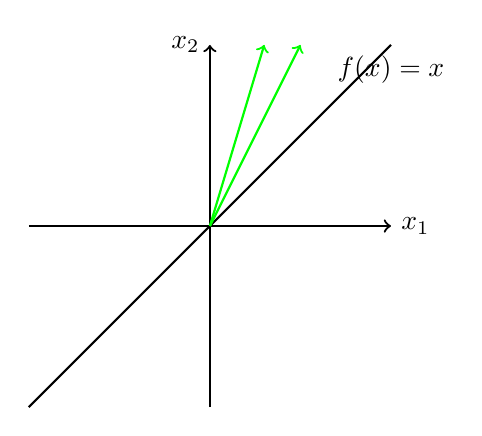
\begin{tikzpicture}[scale=2.3]
\draw[thick,->] (-1,0) -- (1,0) node[anchor=west] {$x_1$};
\draw[thick,->] (0,-1) -- (0,1) node[anchor=east] {$x_2$};
\draw[thick] (0,0) -- (1,1) node[anchor=north] {$f(x) = \abs{x}$};
\draw[thick] (0,0) -- (-1,-1);
\draw[thick,->,color=green] (0,0) -- (0.3,1);
\draw[thick,->,color=green] (0,0) -- (0.5,1);
\end{tikzpicture}
\caption{Representación gráfica de subgradientes.}
\end{figure}

\spart

\spart

Para demostrar que el gradiente es el único subradiente en funciones diferenciables, suponemos que existe un $u$ que no es el gradiente tal que es subgradiente.

\[
    f(\gor{x}+\lambda u) = f(\gor{x}) + \lambda u^\top \grad{f(\gor{x})} + \lambda ||u||R(\gor{x},\lambda u)
\]

Por otro lado, por la definición de subgradiente:

\[
    f(x) \geq f(\gor{x}) + u^\top (x-\gor{x}) \forall x \implies f(\gor{x} + \lambda u) \geq f(\gor{x}) + \lambda ||u||
\]

Restando las 2 ecuaciones y tomando $\lambda \to 0$ deducimos que $||u - \grad{f(\gor{x})}||^2 \leq 0 \implies u = \grad{f(\gor{x})}$

\spart

Hay que distinguir:
\begin{itemize}
 \item subradientes en $\gor{x} = 0 \implies \{u\in \real^n : \norm{u}\leq 1\}$
 \item subgradientes en $\gor{x} \neq 0\implies \rfrac{\gor{x}}{\norm{x}}$.
\end{itemize}

Vamos a ver el primer punto para entenderlo:

\[
    \underbrace{f(x)}_{\norm{x}}\geq \underbrace{f(\gor{x})}_{0} + u^\top (x-\gor{x}) \implies \norm{x} \geq u^\top x
\]

Ahora habría que pensar en el otro caso.

\spart

$\gor{x}$ es solución si $\exists u$ subgradiente tal que $u^\top (x-\gor{x}) \geq 0 \forall x\in S$.
%
Es como siempre, pero con subgradiente para funciones no diferenciables.

\[
    f(x) \geq f(\gor{x}) + \underbrace{u^\top(x-\gor{x})}_{\geq0} \geq f(\gor{x})
\]

Cuando la función es convexa, el recíproco es cierto.
%
La demostración se basa en el teorema del hiperplano soporte.
%
La demostración está en el ¿Mazarak?, un libro de la asignatura de la bibliografía.

\end{problem}


%%%%%%%%%%%%%%%%%%%%%%%%%%%%%%%%%%%%%%%%%%%%%%%%%%%%%%%%%%%%%%%%%%%%%%%%%%%%%%%%%%%
%%%%%%%%%%%%%%%%%%%%%%%%%%%%%%%%%%%%%%%%%%%%%%%%%%%%%%%%%%%%%%%%%%%%%%%%%%%%%%%%%%%
%%%%%%%%%%%%%%%%%%%%%%%%%%%								%%%%%%%%%%%%%%%%%%%%%%%%%%%
%%%%%%%%%%%%%%%%%%%%%%%%%%%		HOJA 5 hoja 5 			%%%%%%%%%%%%%%%%%%%%%%%%%%%
%%%%%%%%%%%%%%%%%%%%%%%%%%%								%%%%%%%%%%%%%%%%%%%%%%%%%%%
%%%%%%%%%%%%%%%%%%%%%%%%%%%%%%%%%%%%%%%%%%%%%%%%%%%%%%%%%%%%%%%%%%%%%%%%%%%%%%%%%%%
%%%%%%%%%%%%%%%%%%%%%%%%%%%%%%%%%%%%%%%%%%%%%%%%%%%%%%%%%%%%%%%%%%%%%%%%%%%%%%%%%%%

\section{Hoja 5}

\begin{problem}[1]

Considera el problema max $x_1+x_2^2+x_3$ sujeto a $x_1^2+x_2^2+x_3^2\leq b$, donde $0<b<1/2$.

\ppart Resuélvelo en función de $b$ utilizando las condiciones $KKT$.

\ppart Sea $F(b)$ la función que da el valor objetivo óptimo en función de $b$. ¿Qué relación existe entre esta función y los multiplicadores de $KKT$?


\solution

Lo primero es escribir el problema en forma estándar:
\begin{ioprob}
\goal{$\min -x_1+x_2^2-x_3$}
\restrictions{$x_1^2+x_2^2+x_3^2-b≤0$}{$0<b<\rfrac{1}{2}$}{}{}{}{}
\end{ioprob}

\spart Escribimos el sistema:

\[
	\begin{array}{r}
		-1+2ux_1 = 0\\
		-2x_2+2ux_2 = 0\\
		-1+2ux_3 = 0\\
		u[x_1^2+x_2^2+x_3^2-b] = 0\\
		x_1^2+x_2^2+x_3^2≤b\\
		u≥0
	\end{array}
\]

Si la restricción no está activa, tenemos $u=0 \implies -1 = 0 \implies $ no puede no ser activa, con lo que:

\[x_1^2+x_2^2+x_3^2 = b\]


Seguimos resolviendo el sistema.
%
Utilizando las ecuaciones $1$ y $3$:

\[
	x_1 = x_3 = \frac{1}{2u} \implies 2x_2(u-1) = 0 \implies x_2 = 0 \vee u = 1
\]

Desglosamos las 2 posibilidades:

\begin{itemize}
	\item[$x_2=0$] Tomando $x_2 = 0 \implies 2x_1^2 = b \to x_1=x_2=\sqrt{\rfrac{b}{2}}$.
%
De las 2 raíces, tenemos que elegir la positiva porque $u≥0$.

	\item[$u=1$] La otra posibilidad es $u=1$, con lo que 
	\[
		u=1\to x^2_2=b-\rfrac{1}{2} < 0 \;\;\; \impliedby \left[b\in\left(0,\rfrac{1}{2}\right)\right]
	\]
\end{itemize}

\paragraph{Conclusión:} 

\[
	\KKT{\sqrt{\rfrac{b}{2}},0,+\sqrt{\rfrac{b}{2}}}
\]

\obs No hay ningún punto factible\marginpar{Hacer la cuenta para comprobarlo} en el que no se cumpla la cualificación de las restricciones y por lo tanto, todos los mínimos son $KKT$, con lo que esta es la solución del problema (por el teorema \ref{thm:cualificacionYKKT})

\spart 

\[
	F(b) = 2\sqrt{\rfrac{b}{2}} = \sqrt{2b}
\]

En el caso lineal, tenemos demostrado para problemas lineales:

\begin{ioprob}
\goal{$\min c^\top x$}
\restrictions{$Ax=b$}{$x≥0$}{}{}{}{}
\end{ioprob}

Siendo el siguiente su dual:

\begin{ioprob}
\goal{$\max b^\top u$}
\restrictions{$A^\top u≤c$}{}{}{}{}{}
\end{ioprob}

Teníamos que $\dpa{z}{b_i} = \gor{u_i}$. ¿Ocurre esto también en problemas no lineales? Vamos a verlo:

\[
	F'(b) = \frac{1}{\sqrt{2b}} = u
\]

\obs Esto no es casualidad.
%
Lo que ocurre para problemas lineales ocurre también para problemas no lineales. 

Esto además puede darnos una intuición sobre porque no hay restricción de signo para multiplicadores correspondientes a restricciones de igualdad. 
Al ser de igualdad, no sabemos qué puede ocurrir al aumentar los recursos.
%
Puede aumentar el multiplicador o reducirse.
En cambio, en los multiplicadores asociados a problemas de desigualdad, es decir, en forma canónica, existe la restricción de signo porque al aumentar los recursos, nos acercamos a las restricción. 


\end{problem}




\begin{problem}[2]

Sean $f$ y $g_i$ ($i=1,\ldots,m$) funciones con derivadas parciales continuas en $\mathbb{R}^n$.

Consideremos el problema
\begin{ioprob}
%\tag{$(P)$}
\goal{$\min f(x)$}
\restrictions{$g_i(x) = 0\; ∀i = 1,...,m$}{}{}{}{}{}
\end{ioprob}

Sea $\overline{x}\in\mathbb{R}^n$ un punto factible para (P)
tal que existen n\'umeros reales $\lambda_1,\ldots,\lambda_m$
para los  que
\[
\nabla f(\overline{x})+\sum_{i=1}^m\lambda_i
\nabla g_i(\overline{x})=0.
\]
Supongamos que $f$ es convexa, $g_i$ es convexa si $\lambda_i>0$
y $g_i$ es c\'oncava si $\lambda_i<0$.
%
Demuestra que
$\overline{x}$ es un m\'{\i}nimo global de (P).

\solution

Reescribimos las hipótesis del problema:

\[
	\grad_x L(\vx,\vec{λ}) = 0
\]
\[
	L(\vx,\vec{λ}) \text{ es convexa en } \vec{x} \text{ por ser combinación lineal positiva de convexas}
\]


Si tengo una función convexa cuyo gradiente se anula $\implies$ se alcanza el mínimo en el punto en el que se anula el gradiente.

\paragraph{Conclusión:}

\[
	f(\gvx) = L(\vx,\vec{λ}) ≤ L(\vx,\vec{λ}) = f(x) \text{ (si } \vx,\gvx \text{ es factible)}
\]
\end{problem}

\begin{problem}[3]

Considera el problema:

\begin{ioprob}
\goal{$\min x_1+x_2-x_3$}
\restrictions{$x_1^2+x_2^2+x_3^2≤27$}{$x_1+x_2≤10$}{}{}{}{}
\end{ioprob}

\ppart Calcula todos los puntos que satisfacen las condiciones $KKT$ correspondientes al problema anterior.

\ppart ¿Podemos asegurar que los puntos calculados en el apartado anterior son mínimos globales del problema? ¿Existe algún mínimo global que no verifique las condiciones $KKT$?

\solution

\spart 

Vamos a calcular los puntos que cumplen las condiciones $KKT$, escribiendo el sistema y resolviéndolo:

\[
	\begin{array}{r}
		1+2u_1x_1 + u_2 = 0\\
		1+2u_1x_2 + u_2 = 0\\
		-1+2u_1x_3 = 0\\
		u_1(x_1^2+x_2^2+x_3^2-27) = 0\\
		u_2 (x_1+x_2-10) = 0
	\end{array}
\]

En este caso vamos a resolverlo informalmente.

$u_1 = 0 \to 0 = -1$\footnote{por la tercera ecuación}, con lo que $u_1 ≠ 0 \to x_1^2+x_2^2+x_3^2 = 27$, es decir, la primera restricción tiene que ser activa. 
Las 2 restricciones no pueden darse al mismo tiempo.
	\[x_1+x_2 = 10\to (-x_2+10)^2+x_2^2+x_3^2=27 \to ... \to \text{ imposible}\]

Con esto, se deduce que 
\[u_2 = 0 \to x_1 = x_2 = \rfrac{-1}{2u_1}\]

Utilizando la tercera ecuación y estos resultados, tenemos $x_3 = \rfrac{1}{2u_1}$.

Recapitulando, tenemos: $x_1 = x_2 = -x_3 = \rfrac{-1}{2u_1}$.
%
Utilizando la restricción activa que relaciona estos 3 valores, tenemos:

\[
	3x_1^2 = 27 \to x_1 = x_2 = \pm 3 = -x_3
\]

De las 2 posibilidades elegimos la negativa, para que concuerde con el signo de $x_1 = x_2 = -3 \to u_1 = -\rfrac{-1}{6} = \rfrac{1}{6} ≥ 0$.
Si hubiéramos elegido la negativa, llegaríamos a un multiplicador negativo, siendo éste el correspondiente a una restricción con desigualdad, lo que no es posible.

\paragraph{Conclusión:}

\[\KKT{-3,-3,3}\]

\spart 

Bajo condiciones de convexidad, KKT es suficiente (\fref{thm:convKKT}).

¿Hay más mínimos globales?
Teníamos también que si se cumple la cualificación de las restricciones, KKT es suficiente.

Vamos a verlo con la cualificación de las restricciones que es más fácil de probar:

\[
	\begin{array}{l}
		\grad f_2(x_1,x_2,x_3) = (1,1,0)\\
		\grad f_1(x_1,x_2,x_3) = (2x_1,2x_2,2x_3)
	\end{array}
\]

No se puede verificar la cualificación si $x_1 = x_2$ y $x_3 = 0$ porque estamos fuera de las restricciones:

\[
\left.\begin{array}{l}
	\left.
	\begin{array}{r}
		x_1+x_2 = 10\\
		x_1=x_2
	\end{array}\right\}\implies x_1=x_2=5\\
	x_1^2+x_2^2+x_3^2 = 27
\end{array}
\right\}\implies 5^2+5^2+0^2 ≠ 27
\]

\paragraph{Conclusión:}

Sólo hay un mínimo global porque ningún punto cumple la cualificación de las restricciones.
%
Los únicos mínimos locales que puede tener el problema son los que cumplen $KKT$, y como sólo hay uno, éste tiene que ser global.

\end{problem}

\begin{problem}[4]

Considera el problema 
\[
\mbox{max}\ x^2_1+2x^2_2-6x_1 \ \mbox{s.a.}\ \ x_1+x_2\geq 1.
\]
\ppart Calcula todos los puntos que satisfacen las condiciones KKT correspondientes al problema anterior.
\ppart ¿Podemos asegurar que los puntos calculados en el apartado anterior son máximos globales del problema? ¿Existe algún máximo global que no verifique las condiciones KKT?

\solution

\spart 

\[\KKT{3,0} \; u=0\]

\[\KKT{\rfrac{5}{3},\rfrac{8}{3}}\; u = \rfrac{8}{3}\]

\spart Como la función no es convexa, el problema no es convexo con lo que las condiciones no son suficiente.

\obs Además, podríamos habernos dado cuenta de que el problema no es acotado, con lo que no existe un máximo global.

Con este razonamiento podríamos contestar a la segunda pregunta.
%
Por si acaso no nos hemos dado cuenta de que no es un problema acotado, podríamos razonar de la siguiente manera:
%
Como todos los puntos cumplen la cualificación de las restricciones, aplicando el teorema correspondiente, tenemos que mínimo local $\implies$ KKT, con lo que son necesarias.

\end{problem}

\obs Este problema estuvo en el examen del año pasado.
\begin{problem}[5]
Sea $f:\mathbb{R}^2\to\mathbb{R}$ convexa y diferenciable.
%
Considera el problema

\begin{ioprob}
\goal{$\min f(x_1,x_2)$}
\restrictions{$x_2-x_1≤0$}{}{}{}{}{}
\end{ioprob}

Supongamos que el problema tiene solución factible óptima.

\ppart Escribe las condiciones de Karush-Kuhn-Tucker (KKT) correspondientes al problema anterior. ¿Qué condiciones debe cumplir $\nabla f(x_1,x_2)$ para que el punto $(x_1,x_2)$ verifique las condiciones KKT? Distingue los casos $x_1=x_2$ y $x_1\neq x_2$.

\ppart Determina razonadamente si son verdaderas o falsas las  afirmaciones siguientes: 

	\begin{itemize}	
		\item Si un punto verifica las condiciones KKT entonces es la solución factible óptima de este problema.
		
		\item La solución factible óptima de este problema podría no verificar las condiciones KKT.
	\end{itemize}


\ppart Si $f(x_1,x_2)=x_1^2+x_2^2+\alpha x_1 + \beta x_2$, donde $\alpha,\beta\in\mathbb{R}$, determina todos los valores de $\alpha$ y $\beta$ para los que la solución del problema tiene sus dos coordenadas iguales. .


\solution

Tenemos:

\[
	\begin{array}{c}
		f'_1(x_1,x_2) - u = 0\\
		f'_2(x_1,x_2) + u = 0\\
		u≥0\\
		x_2-x_1 ≤ 0\\
		u(x_2-x_1) = 0
	\end{array}
\]

Distinguimos los 2 casos que se nos sugieren:

\[x_2 < x_1 \to u = 0 \to \grad f(x_1,x_2) = (0,0)\]

\[x_2 = x_1 \to u ≥ 0 \to  \left\{ 
	\begin{array}{c}
		f_1'(x_1,x_2) ≥ 0\\
		f_2'(x_1,x_2) = - f_1'(x_2,x_2)
	\end{array}\right.
\]

El primer caso está incluido en el segundo. 

\spart 

1) \textbf{Verdadero}, porque al ser un problema convexo de minimización, las condiciones son suficientes para mínimo global.

2) \textbf{Falso}.
%
El gradiente de la restricción no se anula, por lo que todos los puntos factibles verifican la cualificación de las restricciones, con lo que mínimo global  $\implies$ mínimo local $\implies KKT$.


\spart Para que $x_1 = x_2 = t$, tenemos que estar en la frontera.
%
Además, utilizamos las conclusiones del apartado a.

\[
\left.
	\begin{array}{c}
		2t+α≥0\\
		2t+α = -2t-β
	\end{array}
\right\}
\to t = -\frac{α+β}{4} \wedge \frac{-α-β+2α}{2} = \frac{α-β}{2} ≥ 0
\]

Concluimos que $α≥β$.

\obs Si tuviéramos $β<α$, tendríamos el punto en el interior (razonando hacia atrás) y llegaríamos al primer caso de $x_2<x_1$, con lo que tendríamos que igualar el gradiente a $(0,0)$ (como hemos demostrado en el apartado a).

\end{problem}

\begin{problem}[6]

Considera el problema de minimizar $f(x)$ s.a. $f_i(x)\leq 0$, $i=1,\ldots,m$, donde todas las funciones son convexas y diferenciables. 
%
Sean $\bar{x}\in\mathbb{R}^n$ y $\bar{u}\in\mathbb{R}^m$ tales que satisfacen las condiciones KKT. 
%
Demuestra que $\nabla f(\bar{x})^\top (x-\bar{x})\geq 0$, para cualquier punto factible $x$ del problema. 
%
(Sabemos que esta condición implica que $\bar{x}$ es la solución óptima.)


\solution

\proofpart{Fácil}
Como el problema es convexo, KKT es suficiente luego $\gor{x}$ sería un máximo global.

Además, en el tema de convexidad vimos que $\gor{x}$ es un mínimo global $\dimplies \grad f(\gx)^\top (x-\gx) ≥ 0 ∀x$ factible.

\proofpart{Larga}
Sea $\vx$ un punto factible.
%
Por ser factible, $∀i, 0 ≥ f_i(\vx)$.

Por convexidad de $f_i$

\[
	f_i(\vx) ≥ f_i(\gvx) + \grad f_i(\gvx)^\top (\vx-\gvx)
\]

Multiplicamos por los multiplicadores (que son positivos por verificar KKT)

\begin{equation}
\label{5.5.1}
	0 ≥ \sum u_i[f_i(\gvx) + \grad f_i(\gvx)^\top (\vx-\gvx)] \overset{KKT \to u_if_i = 0}{=} \sum u_i\grad f(\gvx)(\vx-\gvx)
\end{equation}


Por $KKT$, también sabemos que se anula el gradiente de la función lagrangiana, es decir:

\[
	\grad f(\gvx) + \sum u_i \grad f_i(\gvx) = 0
\]

Tenemos \ref{5.5.1} $\to -\grad f(\gvx)^\top (\vx-\gvx)$ que es justo lo que nos pedía el enunciado.
\end{problem}

\begin{problem}[7]

Sea $c\in\mathbb{R}^n$, $c\neq 0$. 
%
Considera el problema de maximizar $f(x)=c^\top x$ s.a. 
%
$x^\top x\leq 1$. 
%
Calcula los puntos que verifican las condiciones KKT del problema y determina su máximo global. 

\solution

La solución intuitiva del problema es $\gvx = \rfrac{c}{\norm{c}}$.
%
Vamos a demostrarlo


\begin{ioprob}
\goal{$\min -c^\top x$}
\restrictions{$x^\top x ≤ 1$}{}{}{}{}{}
\end{ioprob}

Escribimos las condiciones:

\[
	\begin{array}{c}
		-c + 2ux = 0\\
		x^\top x≤1\\
		u≥0\\
		u(x^\top x - 1) = 0
	\end{array}
\]

Si $x^\top x - 1$, es decir, estamos dentro de la bola, $\implies u= 0 \implies c=0$, lo que contradice las hipótesis. 
%
Sabemos entonces que la solución está en la frontera, es decir: $x^\top x - 1$.

\[
	x^\top x - 1 \to \norm{x} = 1 
\]

Además,

\todo{revisar cuentas}

\[
	c=2ux'\wedge \norm{c} = 2u \to u = \frac{\norm{c}}{2}>0 \to x = \frac{c}{2u} = \frac{c}{\norm{c}}
\]

\end{problem}


\begin{problem}[8]

Demuestra la desigualdad de dualidad débil ($\bar{d}\leq \bar{p}$) en los casos $\bar{p}=-\infty$ (el problema primal es no acotado) y $\bar{d}=\infty$ (el problema dual es no acotado).


\solution

\ppart Vamos a calcular la función dual:

\[
	g(\vu,\vv) = \inf\{L(\vx,\vu,\vv)\} = \inf \left\{f(\vx) + \sum u_if_i(\vx) + \sum v_ih_i(\vx)\right\} \overset{\vx \text{fact.}}{≤} f(\vx)
\]

Si $u_i ≥ 0$, entonces $g(\vu,\vv) ≤ f(\vx)$.
%
Como $(P)$ no está acotado, deducimos que $g(\vu,\vv) = -∞$, es decir:
%
No hay puntos $(\vu,\vv)$ en el dominio de $g$, o lo que es lo mismo, el problema dual no es factible.

\ppart 

Supongamos que $(P)$ fuese factible.
%
Si el primal es factible, $\exists \gvx$ que cumple las condiciones del $(P)$.

\[
	g(\vu,\vv) ≤ L(\gvx,\vu,\vv) ≤ f(\gvx)
\]

Tenemos una cota superior para algo que no está acotado $\gor{d}$, con lo que no puede existir $\gvx$, es decir, $(P)$ no es factible.

\end{problem}

\begin{problem}[9]

Sean $a_i\in\mathbb{R}^n$, $a_i\in\mathbb{R}^n$, $i=1,\ldots,m$.
%
Considera el problema de minimizar una función lineal a trozos:
\[
\mbox{Minimizar}\ \max_{i=1,\ldots,m} (a_i^\top x + b_i),\ \ x\in\mathbb{R}^n.
\]
Definiendo $y_i=a_i^\top x + b_i$, este problema se puede expresar de forma equivalente como
\begin{center}
\begin{tabular}{ll}
Minimizar & $\displaystyle{\max_{i=1,\ldots,m}} y_i$ \\
sujeto a & \\
& $a_i^\top x + b_i=y_i,\ \ i=1,\ldots,m$
\end{tabular}
\end{center}
Demuestra que el correspondiente problema dual es
\begin{center}
\begin{tabular}{ll}
Maximizar & $b^\top u$ \\
sujeto a & \\
& $A^\top u=0$ \\
& $\mathbf{1}^\top u = 1$\\
& $u\geq 0$,
 \end{tabular}
\end{center}
donde $A$ es una matriz cuyas filas son los vectores $a_1,\ldots,a_m$.
(Conclusión: la minimización de una función lineal a trozos se puede reducir a un problema de optimización lineal.)


\solution
Consultar en las traspas cómo obtener el problema dual del problema lineal. 
%
Los pasos son prácticamente los mismos, aunque se ha resuelto en clase.

\end{problem}


\begin{problem}[10]

Considera el problema:

\begin{ioprob}
\goal{$\min x_1 + x_2$}
\restrictions{$2x_1+x_2-x_3 = 4$}{$x_1+7x_2-x_4= 7$}{}{}{}{}
\end{ioprob}


\ppart Plantea el método de las dos fases con variables artificiales y lleva a cabo una iteración del mismo.

\ppart Resuelve el problema utilizando el algoritmo simplex-dual. 
\solution

Podemos utilizar el método de las 2 fases o el algoritmo del simplex dual.

\proofpart{2 Fases}

\begin{ioprob}
\goal{$\min x_5 + x_6$}
\restrictions{$2x_1+x_2-x_3+x_5 = 4$}{$x_1+7x_2-x_4+x_6 = 7$}{}{}{}{}
\end{ioprob}

La tabla queda:

\begin{table}[hbtp]
\centering
\begin{tabular}{c|cccccc}
&0&0&0&0&1&1\\
\hline
$x_5=4$&2&1&-1&0&1&0\\
$x_6 = 7$&1&\textcolor{blue}{7}&0&-1&0&1\\
\hline
&3&8&-1&0&0
\end{tabular}
\end{table}

El pivote está marcado en azul.

\proofpart{Dual}

\begin{ioprob}
\goal{$\min x_1 + x_2$}
\restrictions{$-2x_1-x_2+x_3 = -4$}{$-x_1-7x_2+x_4 = -7$}{}{}{}{}
\end{ioprob}

Construimos la tabla:

\begin{table}[hbtp]
\centering
\begin{tabular}{c|cccc}
&1&1&0&0\\\hline
$x_3 = -4$&-2&-1&1&0\\
$x_4=-7$&-1&\textcolor{blue}{-7}&0&1\\\hline
&-1&-1&0&0
\end{tabular}
\end{table}

Este es el punto en el que empieza el simplex dual, ya que no ¿hay puntos factibles?

La solución (tras 2 iteraciones) es:

\[
	(x_1,x_2) = \left(\frac{21}{13},\frac{10}{3}\right)
\]

\end{problem}

\begin{problem}[11]

Se dispone de dos complejos vitam\'{\i}nicos (marcas 1 y 2) cuyos costes por unidad de peso son 30 y 40 euros, respectivamente. 
%
Se desea asegurar la ingesta de un m\'{\i}nimo de 36 unidades de vitamina A al d\'{\i}a, 28 unidades de vitamina C y 32 de vitamina D. 
%
Supongamos que la marca 1 proporciona (por unidad de peso) 2 unidades de vitamina A, 2 de vitamina C y 8 de vitamina D.
%
La marca 2 proporciona 3, 2 y 2 unidades respectivamente.

\ppart Plantea el problema de optimizaci\'on para calcular la combinaci\'on de coste m\'as bajo que garantice la ingesta m\'{\i}nima diaria de las tres vitaminas.

\ppart Lleva a cabo una iteraci\'on del algoritmo simplex-dual para resolver este problema.

\solution



\end{problem}


\begin{problem}[12]


Considera el siguiente problema de optimización lineal:

\begin{ioprob}
\goal{$\max 4x_1 + x_2 + 3x_3$}
\restrictions{ $x_1 + 4x_2 \leq 1 $}{$3x_1 - x_2 + x_3 \leq 4$}{$x_i\geq 0,\ i=1,\ldots,3$}{}{}{}
\end{ioprob}


\ppart Escribe el problema en forma estándar. 
%
Escribe la tabla inicial del algoritmo simplex y lleva a cabo una iteración del algoritmo. ¿Se ha alcanzado con esta iteración la solución factible óptima?

\ppart Escribe el problema dual, resuélvelo gráficamente y utiliza la solución del dual para calcular la solución del primal. 

\ppart Escribe la primera tabla del algoritmo simplex-dual y lleva a cabo una iteración del algoritmo. ¿Se ha alcanzado con esta iteración la solución factible óptima?


\solution



\end{problem}

\begin{problem}[13]


Considera el problema
\[
\mbox{Minimizar}\ x^2+1,\ \ \mbox{s.a.}\ (x-2)(x-4)\leq 0.
\]

\ppart Determina el conjunto factible, el valor óptimo y la solución factible óptima del problema.

\ppart Calcula la correspondiente función dual.

\ppart Plantea y resuelve el problema dual. ¿Hay dualidad fuerte? ¿Se verifica la condición de Slater?

\solution

\spart 


\begin{figure}[hbtp]
\centering
\begin{tikzpicture}
\draw[thick,->] (-1,0) -- (6,0) node[anchor=west] {$x$};
\draw[thick,->] (0,-1) -- (0,6) node[anchor=east] {$y$};
\draw (-.5,.25) parabola bend (0,0) (2,4) node[below right] {$x^2$};

\end{tikzpicture}
\end{figure}

\[\gor{x} = 2\;\;\gor{p} = 5\]

\spart 

\[L(\vx,\vu) = x^2+1+u(x-2)(x-3) = (1+u)x^2-6ux+(1+8u)\]

La función dual:

\[
g(\vu) = \inf L(\vx,\vu) = 
	\left\{
		\begin{array}{lcc}
			-∞ & \text{si} & u≤-1\\
			\frac{9u-u^2+1}{1+u} & \text{si} & u>-1
		\end{array}
	\right.
\]


Entonces, el problema dual es:

\begin{ioprob}
\goal{$\max \frac{9u-u^2+1}{1+u}$}
\restrictions{$u≥0$}{}{}{}{}{}
\end{ioprob}

Tomando $\gor{u} = 2$,  tenemos $\gor{d} = g(2) = 5$. 
%
Comprobamos que se cumple la dualidad fuerte.

\spart Hay dualidad fuerte porque se cumplen  las condiciones de Slater.


\end{problem}


